%%%%%%%%%%%%%%%%%%%%%%%%%%%%%%%%%%%%%%%%%%%%%%%%%%%%%%%%%%%%%%%%%%%%%%%%%%%%%%%%
% PARAMETROS DEL DOCUMENTO Y PAQUETES %
%%%%%%%%%%%%%%%%%%%%%%%%%%%%%%%%%%%%%%%%%%%%%%%%%%%%%%%%%%%%%%%%%%%%%%%%%%%%%%%%
\documentclass[12pt, a4paper]{article} %tamaño mínimo de letra 11pto.

\usepackage{graphicx} 
\usepackage[english]{babel} %ingles 
\usepackage[utf8]{inputenc} %Para poder poner tildes
\usepackage{vmargin} %Para modificar los márgenes
\setmargins{2.5cm}{1.5cm}{16.5cm}{23.42cm}{10pt}{1cm}{0pt}{2cm}
%margen izquierdo, superior, anchura del texto, altura del texto, altura de los encabezados, espacio entre el texto y los encabezados, altura del pie de página, espacio entre el texto y el pie de página
\usepackage{caption}
\usepackage{subcaption}
\usepackage{imakeidx}
\usepackage{stmaryrd}
\usepackage{hyperref}
\usepackage{amsmath}
\usepackage[export]{adjustbox}
\usepackage{fancyhdr}
\usepackage{float}
\makeindex

\usepackage{wrapfig}
\usepackage{amsthm, amssymb}

\usepackage{svg}
\usepackage{soul}
\usepackage[none]{hyphenat}

\usepackage{caption}

\usepackage{setspace}
\spacing{1.5}

\begin{document}

\setlength{\parindent}{8pt}

\pagestyle{empty}

%%%%%%%%%%%%%%%%%%%%%%%%%%%%%%%%%%%%%%%%%%%%%%%%%%%%%%%%%%%%%%%%%%%%%%%%%%%%%%%%
% PORTADA %
%%%%%%%%%%%%%%%%%%%%%%%%%%%%%%%%%%%%%%%%%%%%%%%%%%%%%%%%%%%%%%%%%%%%%%%%%%%%%%%%

\begin{titlepage}

{\includesvg[width=1\textwidth]{figures/logos.svg}} %Para ajustar la portada a una sola página se puede reducir el tamaño del logo
\vspace{1cm}

\centering
{ \bfseries \Large UNIVERSIDAD POLITÉCNICA DE MADRID}
\vspace{2cm}

{ \Large MÁSTER EN BIOLOGÍA COMPUTACIONAL}
\vspace{2cm}

{\Large Computational tool for monitoring the cellular nucleus activity}\vspace{2cm}

{\bfseries \LARGE Ángela Vales Estepa}\vspace{2cm}

{\Large Directors: Francisco Monroy Muñoz y Horacio López Menéndez}\vspace{20mm} 

{\large Curso acad\'emico 2020-21}\vspace{5mm} 

\end{titlepage}
\newpage

%%%%%%%%%%%%%%%%%%%%%%%%%%%%%%%%%%%%%%%%%%%%%%%%%%%%%%%%%%%%%%%%%%%%%%%%%%%%%%%%
% ABSTRACT %
%%%%%%%%%%%%%%%%%%%%%%%%%%%%%%%%%%%%%%%%%%%%%%%%%%%%%%%%%%%%%%%%%%%%%%%%%%%%%%%%

{\bfseries \Large Abstract }\vspace{5mm} 

\vspace{1cm}

\newpage

%%%%%%%%%%%%%%%%%%%%%%%%%%%%%%%%%%%%%%%%%%%%%%%%%%%%%%%%%%%%%%%%%%%%%%%%%%%%%%%%
% INDEX %
%%%%%%%%%%%%%%%%%%%%%%%%%%%%%%%%%%%%%%%%%%%%%%%%%%%%%%%%%%%%%%%%%%%%%%%%%%%%%%%%

\tableofcontents
\setcounter{tocdepth}{2}
\newpage

\setcounter{page}{1}
\pagestyle{fancy}
\rhead{Introduction}
\lhead{ }
\renewcommand{\headrulewidth}{0.005pt}

%%%%%%%%%%%%%%%%%%%%%%%%%%%%%%%%%%%%%%%%%%%%%%%%%%%%%%%%%%%%%%%%%%%%%%%%%%%%%%%%
% INTRODUCTION %
%%%%%%%%%%%%%%%%%%%%%%%%%%%%%%%%%%%%%%%%%%%%%%%%%%%%%%%%%%%%%%%%%%%%%%%%%%%%%%%%
\setlength{\parskip}{0mm}

\section{Introduction}

%%%%%%%%%%%%%%%%%%%%%%%%%%%%%%%%%%%%%%%%%%%%%%%%%%%%%%%%%%%%%%%%%%%%%%%%%%%%%%%%
\subsection{Cell nucleus structure and mechanical properties}
%%%%%%%%%%%%%%%%%%%%%%%%%%%%%%%%%%%%%%%%%%%%%%%%%%%%%%%%%%%%%%%%%%%%%%%%%%%%%%%%

All life forms are composed of at least one cell \cite{mazzarello1999unifying} and according to the organism, these cells are either prokaryotic or eukaryotic \cite{vellai1999origin}. Although both cells have differences such as the lack of organelles like mitochondria \cite{keeling2008organelle} and endoplasmic reticulum \cite{rapoport2007protein} in prokaryotic cells, they have one important feature in common, they contain genetic information. However, they do not store the genetic information in the same way, since in the eukaryotic cell it is in the nucleus of the cell, whereas in the prokaryotic cell it is located in the cytoplasm \cite{cook1983mucus}.

\setlength{\parskip}{4mm}

Therefore, the nucleus in eukaryotic cells is important as it contains genetic information stored as nucleic acids, which are replicated and transmitted to daughter cells and control cellular activities \cite{ossareh2001protein}. In addition, the nucleus has relevant structure and mechanical properties, which is essential for cellular functions. Nuclear deformations that occur during cell compression or stretching can modify cell function. Neutrophils, for example, have lobulated nuclei that increase their physical plasticity, allowing them to pass through a narrow tissue space \cite{hoffmann2011integrin}.

In other cases, cell function may be damaged due to defects that change cellular properties \cite{lammerding2011mechanics}. Mutations in genes that encode the nuclear envelope protein lamin A/C, which change some of the mechanical properties of the cell nucleus, cause diseases in humans such as congenital muscular dystrophy, and even in some cases the change in nuclear properties due to the mutation also has a negative impact, worsening the disease \cite{lammerding2004lamin}. Another disease that also causes changes not only in the mechanical properties of the nucleus, but also in the properties of the whole cell, is cancer \cite{jacobs2012introduction, lekka2019measuring, cross2007nanomechanical}.

However, nuclear proprieties are constantly changing in the cells as the cell cycle nucleus undergoes different tasks and conformations that require the progressive remodelling of its microstructure, taking from a decondensed phase where the DNA is accessible for transcription and duplication to the fully condensed phase associated with the paking of the chromosomes towards cell division \cite{liu2017mitosis}.

\newpage

Because of the relationship of the mechanical properties of the nucleus with cell function, cell cycle, and several diseases in humans, the mechanical properties are sought to be determined. There are several techniques to determine the mechanical properties of the cell nucleus. One technique is micropipette aspiration, which studies the properties of the nucleus by aspiration, but it is an invasive technique and the nucleus can be damaged \cite{gonzalez2019advances}. Other technique is atomic force microscopy, which is used to measure the identation in the nucleus of an adherent cell. The problems are the dependence on the probe and the material to which the cell is attached \cite{janel2019stiffness}. Another similar technique is substrate strain, used to measure the stiffness of the nucleus as a function of the deformation of a stretched cell. The problem with this technique is that it requires well-attached cells and the study of the adhesion and structure of the cytoskeleton of each cell \cite{murphy2011automated}. Other method that determines the chromatin strength in the nucleus is the active microrheology, in which a bead that can be moved with optical tweezers is inserted into the nucleus. As the beads in active microrheology are quite large compared to the nuclear size (500 to 1000 nm diameter), another alternative is to perform passive microrheology, in which smaller beads (100 nm) are introduced into the nucleus. However, this method has shortcomings such as a high sensitivity to the size of the beads as if they are not embedded enough, they move more than they should, providing incorrect values \cite{lammerding2011mechanics, lammerding2007nuclear, de2007direct}.

 The principle shared by these techniques is the determination of the mechanical properties of the nucleus by using either a single cell or a single nucleus which is perturbed except for microreology. Based on the study of these techniques, a new technique is proposed, nuclear elastography, which shares the measurement of the mechanical properties of the nucleus with an external force applied by beads, as in microreology, but without introducing them into the nucleus. 
 
 \newpage
 
 \setlength{\parskip}{0mm}

%%%%%%%%%%%%%%%%%%%%%%%%%%%%%%%%%%%%%%%%%%%%%%%%%%%%%%%%%%%%%%%%%%%%%%%%%%%%%%%%
\subsection{The use of waves}
%%%%%%%%%%%%%%%%%%%%%%%%%%%%%%%%%%%%%%%%%%%%%%%%%%%%%%%%%%%%%%%%%%%%%%%%%%%%%%%%

The new technique currently under development, called nuclear elastography, takes its name from its similarity to elastography, a technique that measures the stiffness of tissues by propagating mechanical waves \cite{gennisson2013ultrasound}. In this project, to interrogate the nucleus, we will use the propagation of mechanical waves across the nuclear structure.

\setlength{\parskip}{4mm}

To understand why a mechanical wave is useful in the new technique, it is necessary to consider the following points. A force can produce a wave and the behaviour of the generated wave depends on the medium in which it is produced. That is, the medium has a certain transmission velocity and a specified damping, which depend on the Young's modulus, viscosity, and density of the material \cite{achenbach2012wave}. 

Here, it is proposed the use of sound waves propagating through of the chromatin to “visualise” its internal organisation and characterise its mechanical status.

\setlength{\parskip}{0mm}

%%%%%%%%%%%%%%%%%%%%%%%%%%%%%%%%%%%%%%%%%%%%%%%%%%%%%%%%%%%%%%%%%%%%%%%%%%%%%%%%
\subsection{Indentation with optical tweezers}
%%%%%%%%%%%%%%%%%%%%%%%%%%%%%%%%%%%%%%%%%%%%%%%%%%%%%%%%%%%%%%%%%%%%%%%%%%%%%%%%

The induction of waves into the cell nucleus and their detection once they have passed through the nucleus requires the use of equipment capable of moving small objects that act as force carriers and is able to measure the force of the wave once it has passed through the nucleus. 

\setlength{\parskip}{4mm}

One instrument that fits these requirements is the optical tweezers, which is a laser ray capable of trapping microscopic dielectric objects. Because of this, optical tweezers can manipulate cells, organelles and even microscopic polyester beads \cite{novotny1997theory, ombid2020vitro, ashkin1992forces}. In addition, there are optical tweezers that are not only capable of capturing microscopic objects, but can also measure the force captured by these objects \cite{farre2014force}. 

The concept of optical trapping as a mechanical reporter is insightful \cite{ashkin20182018}, thus it is proposed this approach as a noninvasive tool to inspect isolated nuclei and living cells in the future in the range of nanometers and fast readout.

\newpage

By means of an optical trap, it is set a shaking bead placed out of the nucleus to impinge a sound field as a propagation front wave travelling into the nucleus; the trap performing this task is referred to as a shaker trap (ST). Then, it is used as a single trap for detecting wave fading caused by the rigidity of the granular chromatin; this trap is referred to as a tactile trap (TT). Nevertheless, the measured signal by the TT will be very small, so it can be masked by environmental noise. 

\setlength{\parskip}{0mm}

%%%%%%%%%%%%%%%%%%%%%%%%%%%%%%%%%%%%%%%%%%%%%%%%%%%%%%%%%%%%%%%%%%%%%%%%%%%%%%%%
\subsection{Data analysis}
%%%%%%%%%%%%%%%%%%%%%%%%%%%%%%%%%%%%%%%%%%%%%%%%%%%%%%%%%%%%%%%%%%%%%%%%%%%%%%%%

Data obtained from the sensors has environmental noise and the method to remove it is to use a filter. There are different filters depending on the linearity of the model, the assumed distribution and the computational cost that can be assumed. 

\setlength{\parskip}{4mm}

Two suitable filters in the first filtering step are the low pass and high pass finite impulse response filters. These filters allow selecting from which frequency or up to which frequency to attenuate, so that if a specific frequency is being worked on and there is noise at higher frequencies, these signals can be attenuated by the low pass FIR filter \cite{rabiner1973approximate}, and if the noise occurs at frequencies lower than the working frequency, it is reduced with the high-pass FIR filter \cite{mondal2012novel}.

Then, a frequent filter that is used not only to remove noise from measurements, but also to determine variables that cannot be measured directly is the Kalman filter. This filter is used in Terrain-referenced navigation (TRN) \cite{kim2018introduction}, and single target tracking systems in airborne radar \cite{pearson1974Kalman}. 

The Kalman filter has two stages, the first is the initial stage, in which the values of the state variables are predicted, while the second stage corrects the values, which are determined according to the values collected by the sensor and the estimates, giving a higher weight to the one with the lowest covariance. An important limitation of this filter is that it only works for a linear model. If the model is not linear, the Extended Kalman filter is used. This filter makes nonlinear functions linear around the estimated state and differs from the Kalman filter in that Jacobian matrices are used for state prediction and updating \cite{ribeiro2004Kalman}.

Thus, by using the extended Kalman filter coupled with a wave model for prediction, the signal captured by the beads can be analysed.

Pre-filtering the noise in the captured signal is important, as the extended Kalman filter can filter signals with high-frequency noise but not low-frequency noise, as it converges to the estimated parameters before removing the low-frequency noise. In addition, filtering out high-frequency noise results in better parameter estimation, as the estimated state will be easier to achieve.

\setlength{\parskip}{0mm}

%%%%%%%%%%%%%%%%%%%%%%%%%%%%%%%%%%%%%%%%%%%%%%%%%%%%%%%%%%%%%%%%%%%%%%%%%%%%%%%%
\subsection{New sensor design}
%%%%%%%%%%%%%%%%%%%%%%%%%%%%%%%%%%%%%%%%%%%%%%%%%%%%%%%%%%%%%%%%%%%%%%%%%%%%%%%%

Therefore, due to the relationship between the mechanical properties of the nucleus and the cell cycle and some diseases, such as cancer, it has been decided to look for a new technique to determine them. Thus, a new sensor has been designed to determine the mechanical properties of the cell nucleus. For this purpose, previous techniques have been studied, concluding in the use of optical tweezing together with the extended Kalman filter coupled with a wave model. In addition, to improve the estimation of the extended Kalman filter, the data obtained with the optical tweezers were filtered with a low-pass and a high-pass finite impulse response filter. Three approaches have been used for this purpose.
 
\setlength{\parskip}{4mm}

The first approach is the experimental design, in which different cell types have been used to obtain real data with optical tweezers. On one side, it has been worked with phagocytosis of beads in HeLa cells \cite{gey1952tissue} to obtain data with alive cells and on the other side with isolated nuclei of Jurkat cells \cite{schneider1977characterization, gioia2018genome} and isolated nuclei of Jurkat cells incubated with the drug jasplakinolide, so that it can be checked that the algorithm works with different cell parameters and detects the difference between both \cite{andersen2002directed}, since the druga promotes the polymerization  of actin \cite{holzinger2001jasplakinolide}.

The second approach is the computational design in which the extended Kalman filter coupled with a one-dimensional wavelet model has been implemented, and a two-dimensional wavelet model has been developed, which is used for modelling the data used as simulated real data in the tests of the above algorithm.  The use of simulated data is important to be able to perform simulations and determine whether the algorithm works, in which regions and under which conditions and its limitations. A preprocessing routine of the obtained data was also performed to remove noise from the collected experimental data. This is important for a better estimation of states and parameters.

The third approach is to validate that the developed sensor works using the developed algorithm with the real data obtained. 

\newpage
\setlength{\parskip}{0mm}
%%%%%%%%%%%%%%%%%%%%%%%%%%%%%%%%%%%%%%%%%%%%%%%%%%%%%%%%%%%%%%%%%%%%%%%%%%%%%%%%
% METHODS %
%%%%%%%%%%%%%%%%%%%%%%%%%%%%%%%%%%%%%%%%%%%%%%%%%%%%%%%%%%%%%%%%%%%%%%%%%%%%%%%%

\rhead{Methods}
\section{Methods}

To achieve the goal of this work, monitoring the nuclear mechanical parameters, the following methodology presented in the figure \ref{fig:esquema_trabajo} has been carried out.

\begin{figure}[htbp]
  \centering
  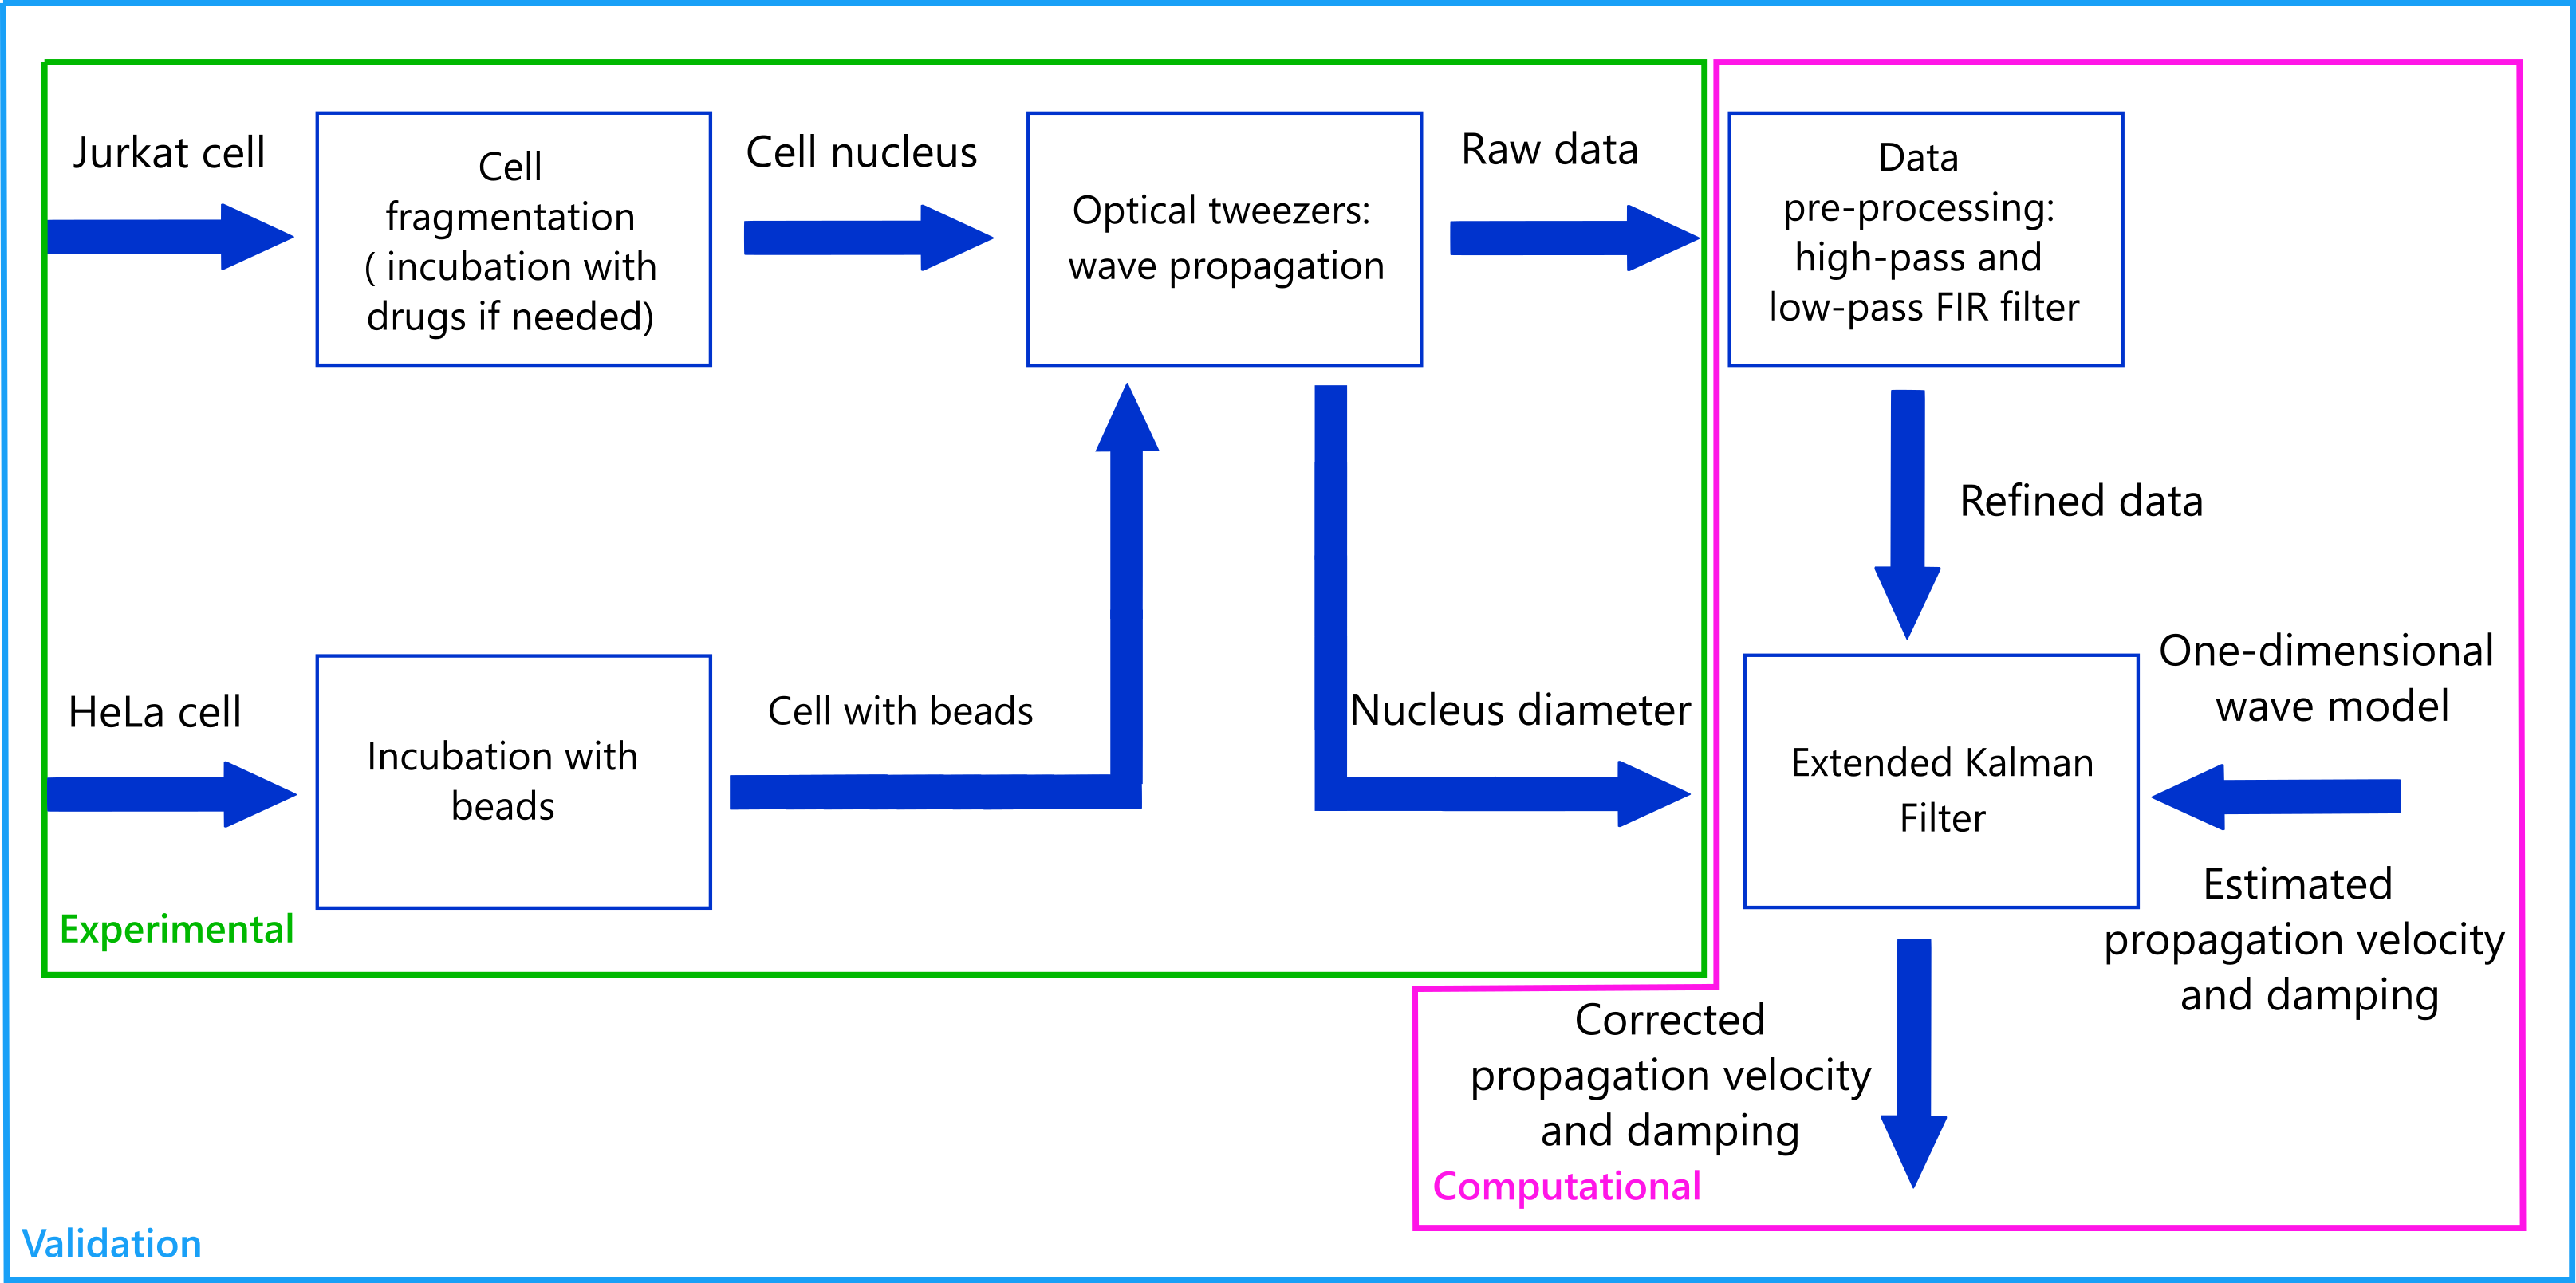
\includegraphics[width=1\textwidth]{figures/esquema_trabajo_metodos_2.png}
  \caption{Block diagram of the process followed to make the new sensor.}
  \label{fig:esquema_trabajo}
\end{figure}

The starting point of the experimental path is the cell, the Jurkat cells were fragmented to obtain their isolated nucleus, which can be used as it was, or after incubation with drugs, in this case jasplakinolide. HeLa cells were not fragmented, but incubated with beads so that they could be phagocytosed and live cell data obtained. Isolated Jurkat cell nuclei in solution with beads and HeLa cells with embedded beads were placed in optical tweezers to oscillate one bead at the edge of the nucleus producing a mechanical wave while the other, located at the other end of the nucleus, captured the force data after crossing the cell nucleus. In addition, while the cell nucleus was in the optical tweezers, a photograph was taken, so that the diameter of the nucleus and thus the distance of the beads could be obtained.

An algorithm was developed to analyse the real data. First, a preprocessing system was performed in which the offset was set and the high and low frequency ambient noise captured by the tactile trap was removed using a high-pass filter and a low-pass finite impulse response filter. Once the data has been filtered, it was introduced into the extended Kalman filter, which provides better parameter estimation with a lower noisy dataset. The extended Kalman filter, coupled to a one-dimensional wave model, with a known nuclear diameter and initially estimated parameters (transmission velocity and damping), corrected these parameters. To check that these algorithms worked, a signal with different frequencies was modelled and a two-dimensional wave model was made, inserting these datasets into the preprocessing and extended Kalman filter respectively.

Once the real data were obtained and the algorithms were verified to work, the sensor validation was started by inputting the real data instead of the simulated data into the algorithms. 

\setlength{\parskip}{0mm}

%%%%%%%%%%%%%%%%%%%%%%%%%%%%%%%%%%%%%%%%%%%%%%%%%%%%%%%%%%%%%%%%%%%%%%%%%%%%%%%%
\subsection{Experimental desing}
%%%%%%%%%%%%%%%%%%%%%%%%%%%%%%%%%%%%%%%%%%%%%%%%%%%%%%%%%%%%%%%%%%%%%%%%%%%%%%%%

%%%%%%%%%%%%%%%%%%%%%%%%%%%%%%%%%%%%%%%%%%%%%%%%%%%%%%%%%%%%%%%%%%%%%%%%%%%%%%%%
\subsubsection{Jurkat cells, cell fragmentation and incubation with drug}
%%%%%%%%%%%%%%%%%%%%%%%%%%%%%%%%%%%%%%%%%%%%%%%%%%%%%%%%%%%%%%%%%%%%%%%%%%%%%%%%

In this study, human Jurkat cells have been used,  which is a human CD4 T-lymphocyte leukaemia cell line \cite{schneider1977characterization}. They were cultured in a humidified atmosphere with 5\% of CO$_{2}$ and 95\% of air at 37ºC. The medium for Jurkat cells was composed of 90\% RPMI 1640 with L-Glutamine (Sigma-Aldrich/USA) and 10\% FBS (Sigma-Aldrich/USA).

\setlength{\parskip}{4mm}

For the isolation of Jurkat cell nuclei, 3ml of the indicated medium with a cell concentration of 3,1$\cdot$10$^5$cells/ml were used. First, the samples were centrifuged in the thermo scientific Micro 21R centrifuge at 2000rpm over 5 minutes. Then, the sobrenadant was discarded and the pellet was resuspended in 300$\mu$l buffer A and 3$\mu$l protease inhibitor cocktail (Sigma-Aldrich/USA) were added. The sample was incubated on ice for 5 minutes and subsequently centrifuged at 8000rpm for 5 minutes at 4ºC. The sobrenadant was removed and the pellet was resuspended with 300$\mu$l buffer A and 3$\mu$l protease inhibitors. It was incubated for 5 minutes on ice and then centrifuged for 5 minutes at 8000rpm at 4ºC in the same centrifuge. Finally, the sobrenadant was removed and the nucleus pellet was resuspended in TKM buffer. This was the stock solution of the cell nucleus.

\newpage

For experiments with drug-incubated nuclei, 3ml of nuclei extracted in TKM solution were used. These 3ml were separated into two samples of 1,50ml each. One of these samples was the control and the other sample with nuclei affected by the drug jasplakinolide. In the sample whose nuclei were affected by jasplakinolide, the nuclei were incubated with the drug at a concentration of 10$\mu$g/ml for 30 minutes at room temperature. To obtain this concentration, 11,11$\mu$l of jasplakinolide at a concentration of 100$\mu$g/ml was added to the 1,50ml sample. The control sample was added 11.11$\mu$l of DMSO, as the jasplakinolide drug was dissolved in this organic solvent, so if it affected the nucleus properties it would not have been attributed to jasplakinolide. The control sample was incubated for 30 minutes as well. Subsequently, both samples were centrifuged with the thermo scientific Micro 21R centrifuge at 8000rpm at 4ºC for 5 minutes. Finally, the sobrenadant was removed and the pellet was resuspended with 150$\mu$l of TKM. Both samples were stock solutions of nuclei, one sample affected by the drug and the other the control.

\setlength{\parskip}{0mm}

%%%%%%%%%%%%%%%%%%%%%%%%%%%%%%%%%%%%%%%%%%%%%%%%%%%%%%%%%%%%%%%%%%%%%%%%%%%%%%%%
\subsubsection{HeLa cells and incubation with beads}
%%%%%%%%%%%%%%%%%%%%%%%%%%%%%%%%%%%%%%%%%%%%%%%%%%%%%%%%%%%%%%%%%%%%%%%%%%%%%%%%

Human HeLa cells have been used, which is a human cervical cancer line \cite{gey1952tissue}. They were cultured in a humidified atmosphere with 5\% of CO$_{2}$ and 95\% of air at 37ºC. The medium for HeLa cells was composed of 90\% DMEM (GIBCO/UK) and 10\% FBS (GIBKO/UK).

\setlength{\parskip}{4mm}

Different methodologies have been used to incubate HeLa cells with beads. First, a cell-culture treated multidishes of 24 dishes was used, and 500$\mu$l of DMEM (GIBCO/UK) and 10$\mu$l of a concentration 3,95 $\times$ 10$^{5}$ cells/ml were added. After 48h, the medium was removed and each dish was filled with new medium and a different percentage of beads of 2.0$\mu$m (Sigma-Aldrich/DE). In the control no beads were added, only 500$\mu$l DMEM, in another dish 500$\mu$l of DMEM with 0,05mg/ml of beads was added and in another one 500$\mu$l of DMEM with 0,1mg/ml of beads was added. After 24 hours, the medium was removed and the cells were washed. For this purpose, 500$\mu$l of PBS with pH 7.4 (GIBKO/UK) was added to each dish and after 3 minutes, PBS was removed and the process was repeated three times for each dish. When the PBS was removed for the last time, the cells were stored with 500$\mu$l of DMEM. These cells were then ready for use. 

Another methodology used was to use individual sterile 60mm X 20mm petri dishes. Cover glasses of 20 mm x 20 mm were inserted into the petri dishes, and here the cells were incubated. 200$\mu$l of DMEM with a concentration of 3,95 cells/ml was added to each plate and 1,50ml of DMEM. After 24 hours, the medium was removed and each dish was filled with new medium and a different percentage of 2.0$\mu$m beads, the control one had no beads and was filled with 1,50ml of DMEM and the other dishes were filled with 0,05mg/ml of beads solution in DMEM. After 24 hours, the medium was removed and the cells were washed, 1,50ml of PBS with pH 7.4 (GIBKO/UK) was added to each dish and after 3 minutes, PBS was removed and the process was repeated three times for each dish. When the PBS was removed for the last time, the cells were stored with 1,50ml of DMEM. These cells were ready.

\setlength{\parskip}{0mm}

%%%%%%%%%%%%%%%%%%%%%%%%%%%%%%%%%%%%%%%%%%%%%%%%%%%%%%%%%%%%%%%%%%%%%%%%%%%%%%%%
\subsubsection{Identation of cell nucleus with optical tweezers}
%%%%%%%%%%%%%%%%%%%%%%%%%%%%%%%%%%%%%%%%%%%%%%%%%%%%%%%%%%%%%%%%%%%%%%%%%%%%%%%%

\begin{wrapfigure}{l}{0.50\linewidth}
	\centering
	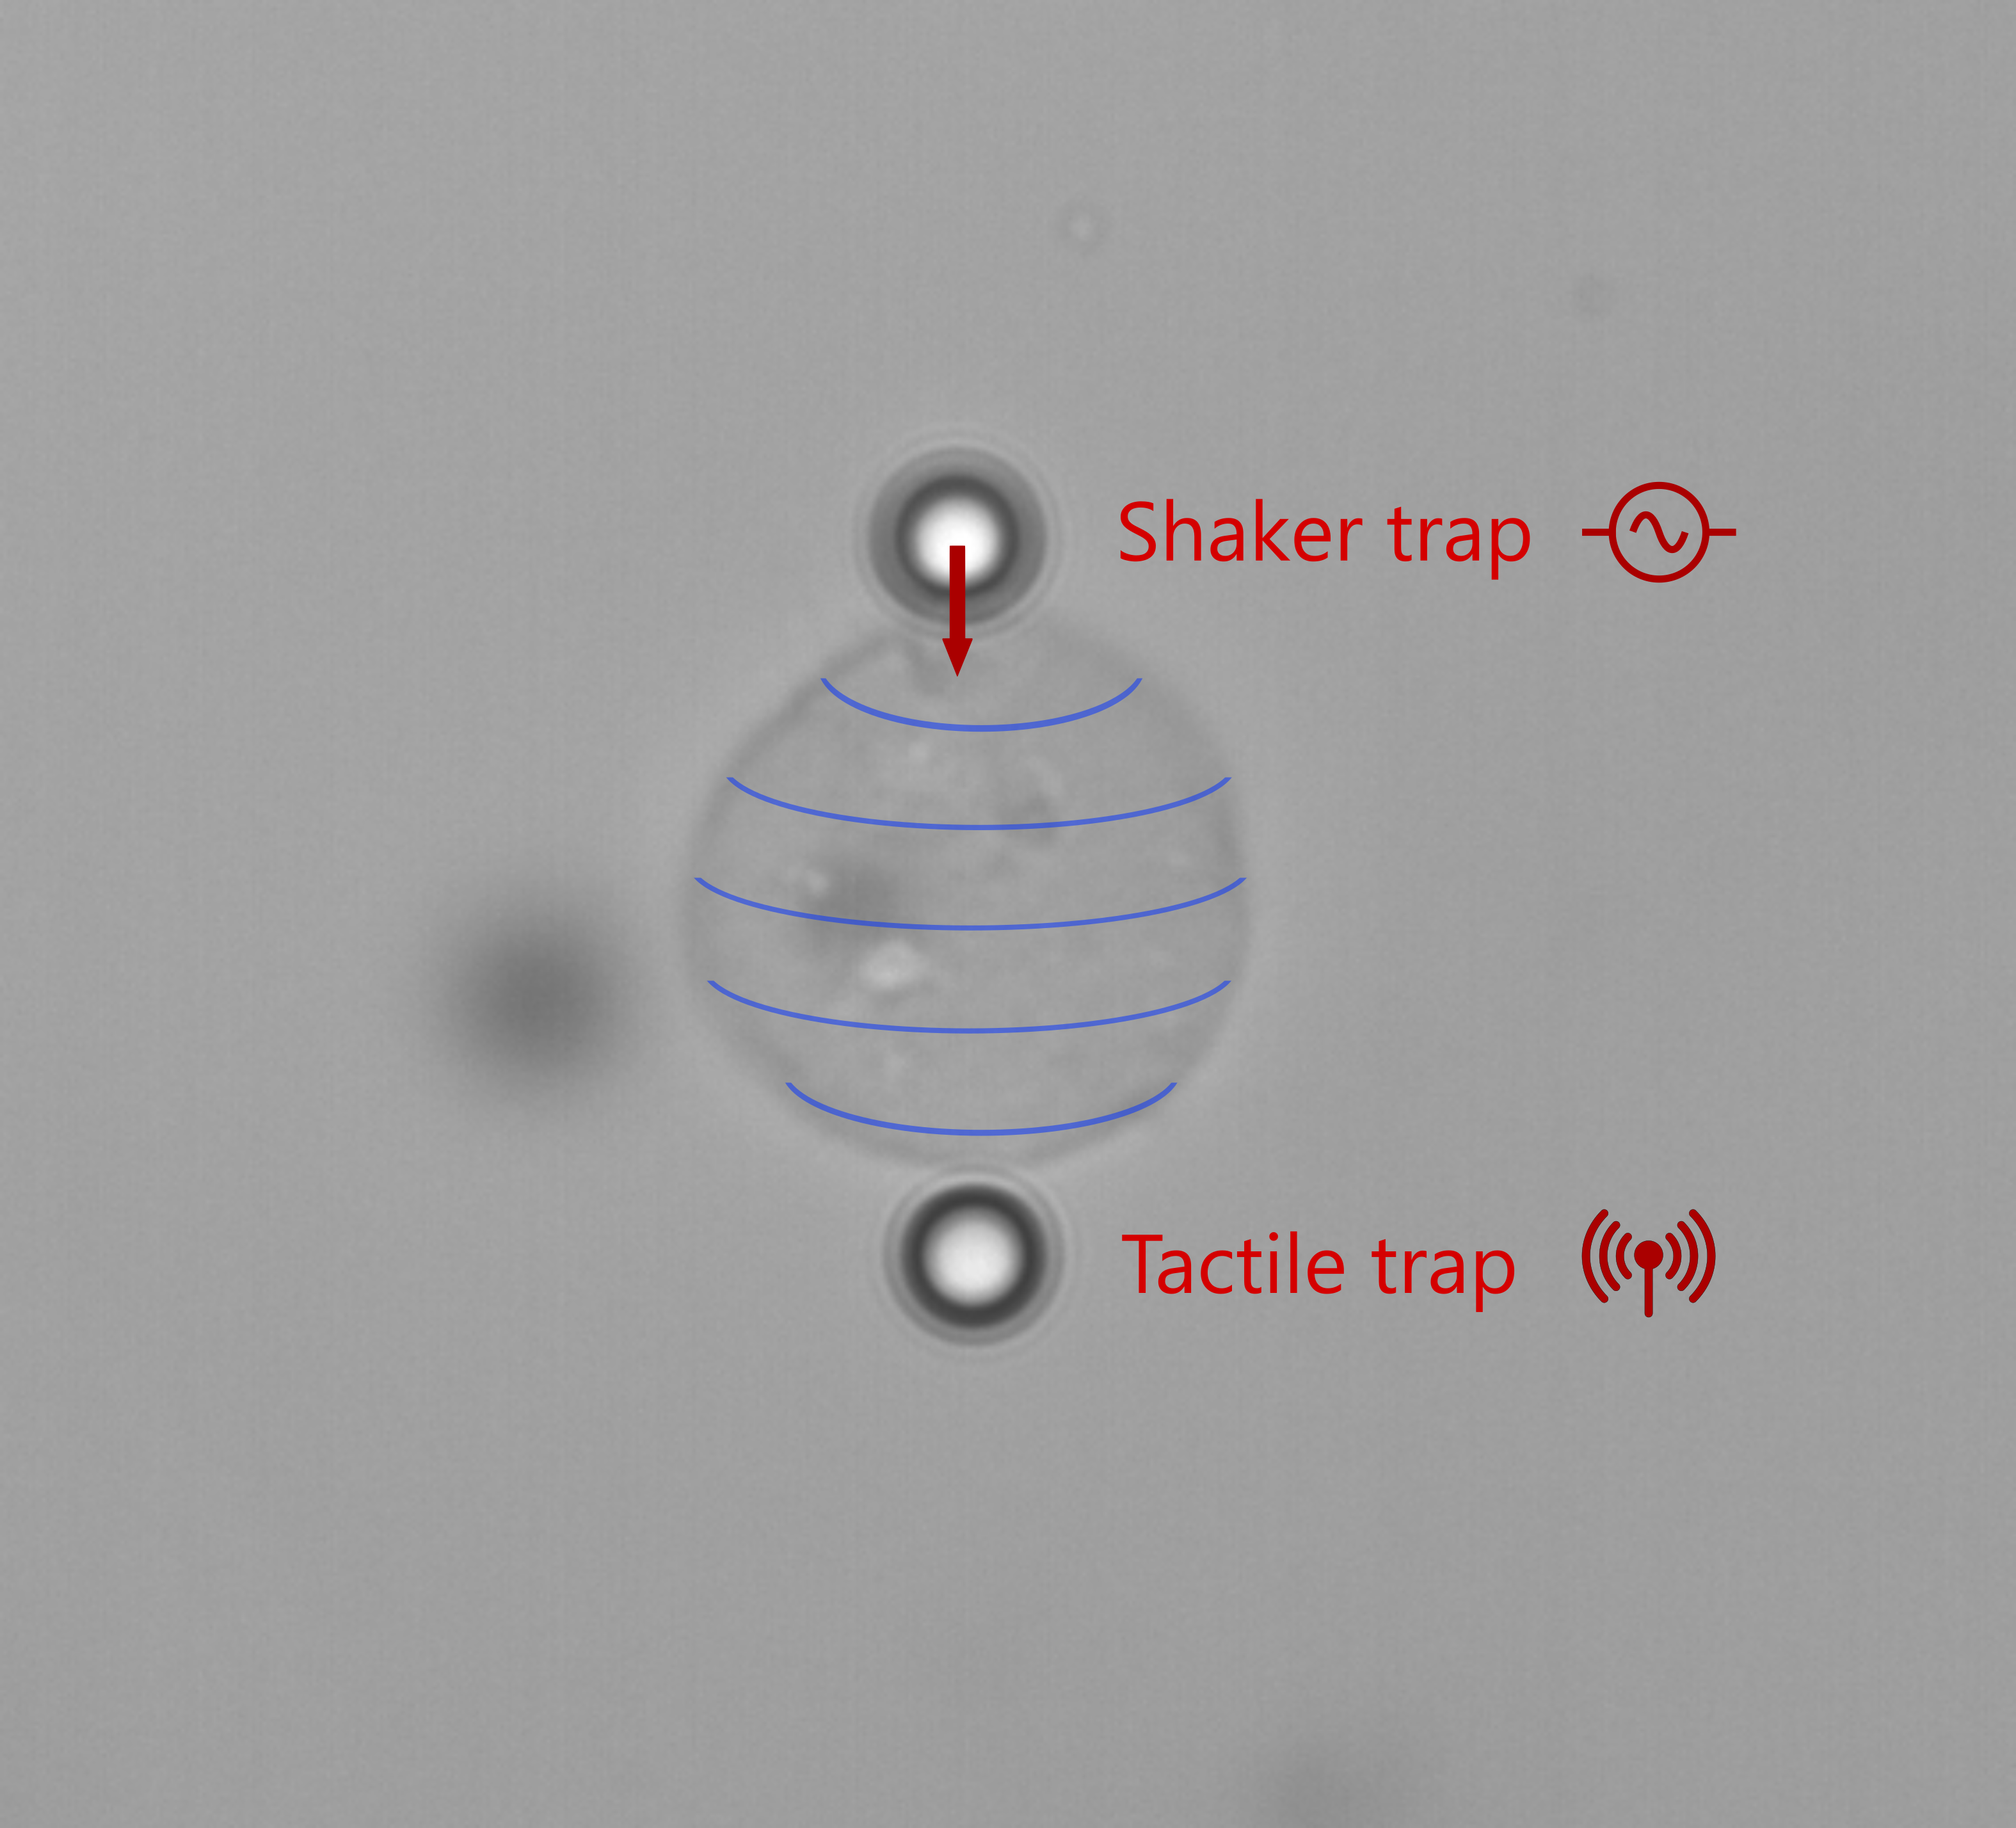
\includegraphics[width=0.45\textwidth]{figures/jurkat_nucleus_waves.png}
	\caption{Isolated Jurkat cell nucleus with two beads (shaker and tactile beads) of size 3mm. The blue lines represent the ideal wave propagation through the nucleus.}
	\label{fig:myfig2}
\end{wrapfigure}

The equipment used were an inverted microscope (Nikon Eclipse 2000Ti) connected with an external light and optical tweezers (Sensocell) coupled with a force sensor. A fast camera (FASCAM SA3-Photron) was used to visualise the sample under the microscope, with which the images presented in the paper were also taken.

\setlength{\parskip}{4mm}

To view it with optical tweezers, a square of double-sided tape with a square cut out inside was cut out. This piece of tape was stuck on a 76 x 26 mm slide (Deltalab/ES) and the cover glass was placed on the top. The sample was placed in the optical tweezers with the glass cover on the bottom.

\setlength{\parindent}{0pt}

\newpage

%%%%%%%%%%%%%%%%%%%%%%%%%%%%%%%%%%%%%%%%%%%%%%%%%%%%%%%%%%%%%%%%%%%%%%%%%%%%%%%%
{\textbf{Isolated Jurkat cell nucleus}}
%%%%%%%%%%%%%%%%%%%%%%%%%%%%%%%%%%%%%%%%%%%%%%%%%%%%%%%%%%%%%%%%%%%%%%%%%%%%%%%%

To perform the indentation on the isolated Jurkat cell nucleus, a dilution of the isolated nuclei was performed in the same day as the nucleus were isolated. To obtain 100$\mu$l of final solution, 65$\mu$l of the isolated nuclei stock, 30$\mu$l of TKM buffer and 5$\mu$l of a 1:100 solution of 3.0$\mu$m beads or 2.0$\mu$m (Sigma-Aldrich/DE) were needed. 40$\mu$l of nuclei solution with beads were poured in the double-sided tape square of the slide and it was covered by a 22 x 40 mm cover glass (Deltalab/ES).

\setlength{\parindent}{8pt}

The sample was focused and a rounded nucleus with no traces of the rest of the cell was looked for. Then, two beads were picked up with optical tweezers and placed on either side of the nucleus. Finally, one bead was oscillated and the position, force and tramp power at each time was collected by both other bead.

\setlength{\parindent}{0pt}

%%%%%%%%%%%%%%%%%%%%%%%%%%%%%%%%%%%%%%%%%%%%%%%%%%%%%%%%%%%%%%%%%%%%%%%%%%%%%%%%
{\textbf{HeLa cells}}
%%%%%%%%%%%%%%%%%%%%%%%%%%%%%%%%%%%%%%%%%%%%%%%%%%%%%%%%%%%%%%%%%%%%%%%%%%%%%%%%

To perform the indentation of HeLa cells there were two ways depending on the incubation method. If HeLa cells have been incubated in cell-culture treated multidishes, the cells have had to be detached (as they are adherent cells) and the dilution of cells with culture medium was placed inside the square of tape. If, on the other hand, they were incubated in individual petri dishes, the cover glas was picked up with tweezers and placed on top of the square of double-sided tape. With these cells, the aim was to find a cell with two embedded beads on opposite sides of the nucleus. Traps were placed on the beads and one of the beads was oscillated while the other one collected the signal after passing through the nucleus.

\setlength{\parindent}{8pt}

\setlength{\parskip}{0mm}

%%%%%%%%%%%%%%%%%%%%%%%%%%%%%%%%%%%%%%%%%%%%%%%%%%%%%%%%%%%%%%%%%%%%%%%%%%%%%%%%
\subsection{Computational desing}
%%%%%%%%%%%%%%%%%%%%%%%%%%%%%%%%%%%%%%%%%%%%%%%%%%%%%%%%%%%%%%%%%%%%%%%%%%%%%%%%

%%%%%%%%%%%%%%%%%%%%%%%%%%%%%%%%%%%%%%%%%%%%%%%%%%%%%%%%%%%%%%%%%%%%%%%%%%%%%%%%
\subsubsection{Preprocessing of the signal}
%%%%%%%%%%%%%%%%%%%%%%%%%%%%%%%%%%%%%%%%%%%%%%%%%%%%%%%%%%%%%%%%%%%%%%%%%%%%%%%%

The data obtained in the experiment required filtering as the installation in which they were obtained was not isolated. In addition to noise, the signal required off-set correction. 

\setlength{\parskip}{4mm}

The purpose of this first preprocessing was not only the preparation of my data, but the development of a script to process all data coming from the optical tweezers. For this reason, the functions have been realised in such a way that it was understandable and segmented, and the only thing that was needed to be entered in the script was the address of the data.

\begin{figure}[htbp]
	\centering
	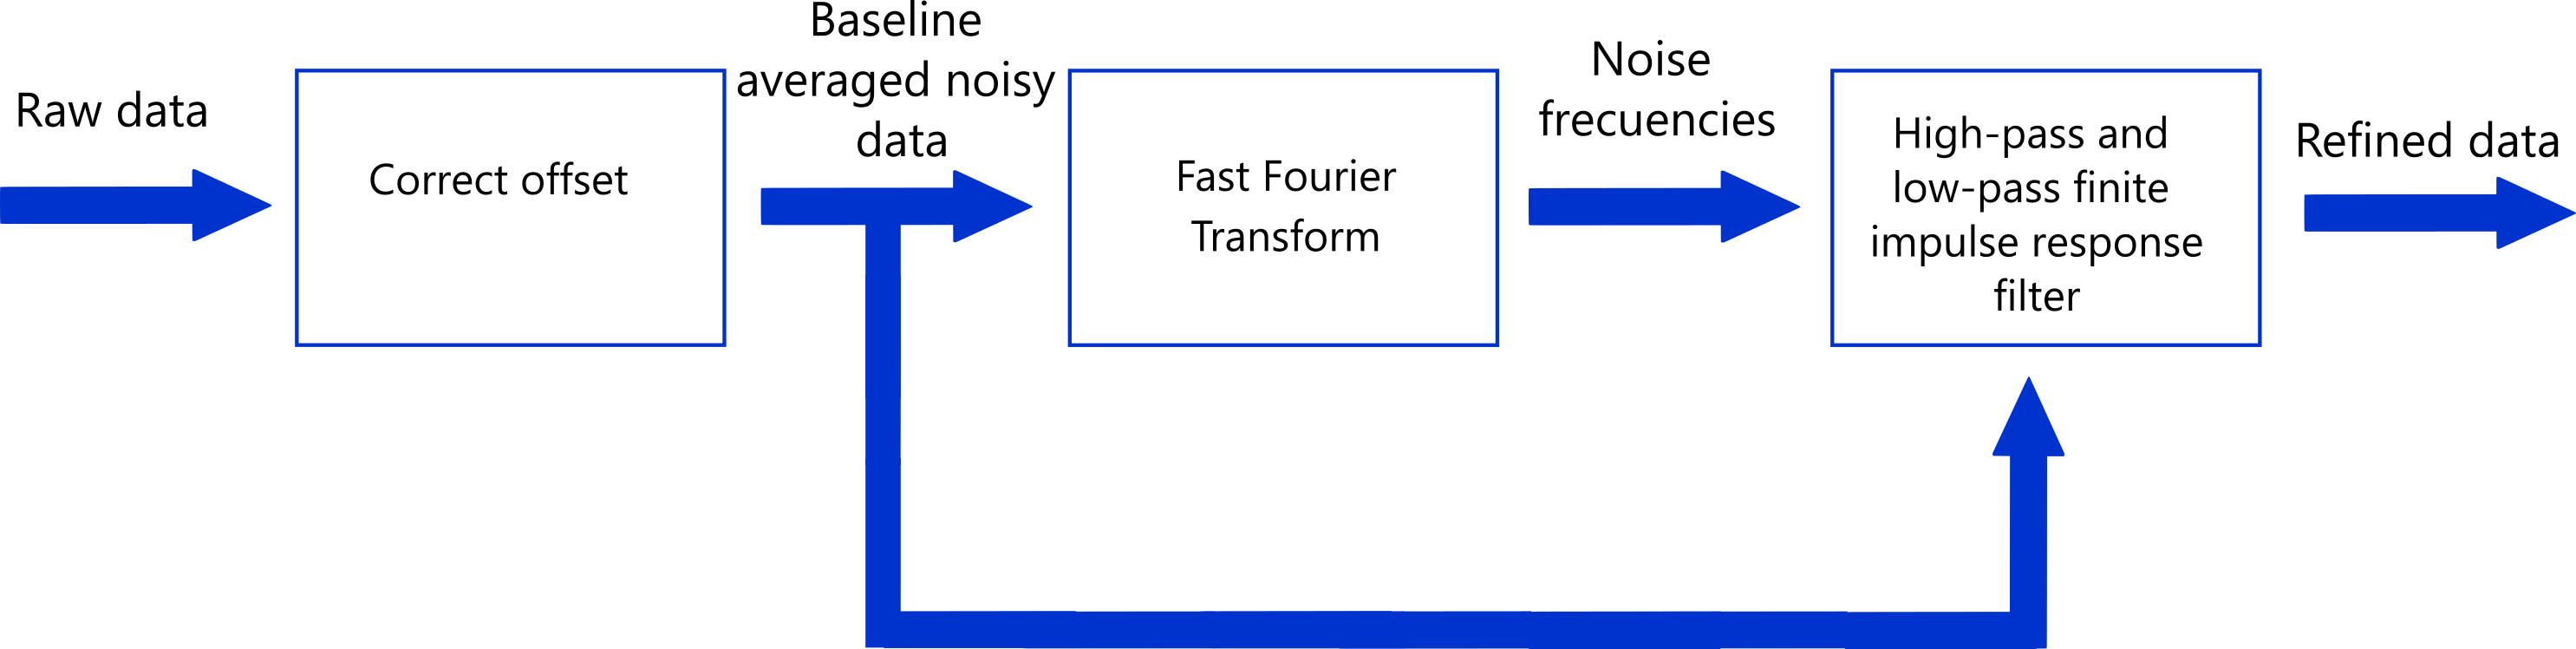
\includegraphics[width=1\textwidth]{figures/esquema_preprocesado_metodos_1.png}
	\caption{Block diagram of data preprocessing}
	\label{fig:esquema_preprocesado}
\end{figure}

To process the data, low-pass and high-pass FIR filters were performed, checking that they worked properly by performing a Fourier transform before and after filtering. 

\setlength{\parskip}{8mm}
\setlength{\parindent}{0pt}

%%%%%%%%%%%%%%%%%%%%%%%%%%%%%%%%%%%%%%%%%%%%%%%%%%%%%%%%%%%%%%%%%%%%%%%%%%%%%%%%
\textbf{Obtain the data and its information and set the off-set}
%%%%%%%%%%%%%%%%%%%%%%%%%%%%%%%%%%%%%%%%%%%%%%%%%%%%%%%%%%%%%%%%%%%%%%%%%%%%%%%%
\setlength{\parskip}{0mm}

Firstly, the address at which the data was stored on the computer was used to obtain both the data and information about the data. Information about this data was obtained from the name of the folder in which it was stored. This was important as it indicated which direction of identation and frequency was used in the experiment and the cell nucleus number. These parameters were interesting for the analysis.

\setlength{\parindent}{8pt}
\setlength{\parskip}{4mm}

The offset of the data was corrected by averaging the values and subtracting that score from each of the values.

\setlength{\parindent}{0pt}
\setlength{\parskip}{8mm}
%%%%%%%%%%%%%%%%%%%%%%%%%%%%%%%%%%%%%%%%%%%%%%%%%%%%%%%%%%%%%%%%%%%%%%%%%%%%%%%%
\textbf{Low and high pass finite impulse response filter}
%%%%%%%%%%%%%%%%%%%%%%%%%%%%%%%%%%%%%%%%%%%%%%%%%%%%%%%%%%%%%%%%%%%%%%%%%%%%%%%%
\setlength{\parskip}{0mm}

The signals captured by the sensors have noise from different sources, high-frequency noise has electromagnetic origin, while low-frequency noise has mechanical origin. A low pass and high pass finite impulse response filter were implemented to remove noise from the signal captured by the sensor \cite{mondal2012novel}. 

\setlength{\parskip}{4mm}
\setlength{\parindent}{8pt}

A high pass FIR filter has been used to reduce low-frequency noise, while low pass FIR filter reduced the noise of high frequencies. For this purpose, the matlab $desingfilt$ function has been used \cite{jacob2015digital}, in which it has been indicated whether it is a high pass or low pass FIR filter with a degree 5, with a passband ripple of 0.2dB and the frequencies filtered are those greater than 5Hz of the frequency with which the bead is identating and less than 1Hz if the frequency with which it has been identated is 2Hz, if the frequency with which it has been identated is less than 7Hz, the frequencies less than 2Hz are filtered, and if it is identated with a frequency greater than 7Hz, all frequencies 5Hz lower than the one used are filtered.

\setlength{\parindent}{0pt}
\setlength{\parskip}{8mm}
%%%%%%%%%%%%%%%%%%%%%%%%%%%%%%%%%%%%%%%%%%%%%%%%%%%%%%%%%%%%%%%%%%%%%%%%%%%%%%%%
\textbf{Fast Fourier transform}
%%%%%%%%%%%%%%%%%%%%%%%%%%%%%%%%%%%%%%%%%%%%%%%%%%%%%%%%%%%%%%%%%%%%%%%%%%%%%%%%
\setlength{\parskip}{0mm}

To verify before and after filtering that the filtering had been performed correctly, the fast Fourier transform was made. The Fourier transform obtains the spectrum of frequencies of a signal. This makes possible to find which frequencies are associated with the noise of a signal, so that it is possible to know which frequencies should be eliminated or which are not recommended to work with \cite{de2001transformada}.

\setlength{\parskip}{4mm}
\setlength{\parindent}{8pt}

To perform the fast Fourier transform in Matlab, the $fft$ function has been used, and as this function reflects the punctual noise and not only the permanent noise in the experiment, the average of the Fourier transform has been performed \cite{shabaninezhad2021matlab}. For this purpose, a series of data were taken in which there are two cycles of oscillations, and these values were averaged. Subsequently, each value was divided by the number of total values, thus the spectrum P2 was obtained. The spectrum P1 is computed from P2 and the length of the signal. Finally, the frequency spectrum is defined and the amplitude of the frequencies is plotted \cite{FourierTransform, frigo1998fftw}.

\setlength{\parskip}{0mm}
%%%%%%%%%%%%%%%%%%%%%%%%%%%%%%%%%%%%%%%%%%%%%%%%%%%%%%%%%%%%%%%%%%%%%%%%%%%%%%%%%%
\subsubsection{Wave model and implementation}
%%%%%%%%%%%%%%%%%%%%%%%%%%%%%%%%%%%%%%%%%%%%%%%%%%%%%%%%%%%%%%%%%%%%%%%%%%%%%%

To interpret the results obtained from the optical tweezers, a one-dimensional polar wave model was implemented in Matlab. This makes the computational cost lower than with a two-wave model, and the energy dispersion is more representative than in a one dimension model with Cartesian coordinates. This model was coupled with the Kalman filter, so in order to verify that it worked, a two-dimensional wave model in Cartesian coordinates was also implemented, obtaining simulated values with which to perform the test. For this purpose, the wave equation with transmitting velocity $c$, damping $d$ and external force $\delta_{Fext}$, was used as a starting point \cite{achenbach2012wave, d'alembert_1749}.

\setlength{\parskip}{4mm}

\begin{equation} \label{eqn:wave_model}
   \frac{\partial^{2}u}{\partial t^{2}} = c^{2}\nabla^{2}u + d\frac{\partial u}{\partial t} + \delta_{Fext}
\end{equation}

The wave equation has been solved by the finite difference method \cite{petter2017finite} with Neumann boundary conditions \cite{mathews2000metodos}. The approximation of some terms was carried out using the finite difference method in the following way:

\begin{equation} \label{eqn:deltau_deltat2}
   \frac{\partial^{2}u}{\partial t^{2}} = \frac{u^{k + 1} - 2u^{k} + u^{k - 1}}{\Delta t^{2}} 
\end{equation}

\begin{equation} \label{eqn:deltau_deltat}
   \frac{\partial u}{\partial t} = \frac{u^{k + 1} - u^{k}}{\Delta t}
\end{equation}

Moreover, the Neumann boundary condition was defined as:

\begin{equation} \label{eqn:neumann}
 \frac{\partial}{\partial N} u(x, y) = 0
\end{equation}

This means that the flow across the edge was 0. To incorporate this into the problem, it has been defined that the border node conditions for a node $u_{n}$ were as follows:

\begin{equation} \label{eqn:neumman_node}
    u_{n-1} = u_{u+1}
\end{equation}

The force was defined by the following equation:

\begin{equation} \label{eqn:force}
    \delta_{Fext} = Asin(wt) = Asin(f2\pi t)
\end{equation}

The amplitude was noted as $A$, the angular velocity as $w$ and the time as $t$, furthermore the angular velocity was replaced by the frequency $f$ multiplied by $2\pi$. The implementation of the wave model has been carried out according to the following procedure.

\setlength{\parindent}{0pt}

\setlength{\parskip}{8mm}

%%%%%%%%%%%%%%%%%%%%%%%%%%%%%%%%%%%%%%%%%%%%%%%%%%%%%%%%%%%%%%%%%%%%%%%%%%%%%%%%
\textbf{One-dimensional wave model}
%%%%%%%%%%%%%%%%%%%%%%%%%%%%%%%%%%%%%%%%%%%%%%%%%%%%%%%%%%%%%%%%%%%%%%%%%%%%%%%%
\normalsize 

\setlength{\parskip}{0mm}

The wave equation (\ref{eqn:wave_model}) was solved in polar coordinates with the Neumann boundary condition and the finite difference method on a node grid in one dimension. 

\setlength{\parindent}{8pt}
\setlength{\parskip}{4mm}

The squared gradient of u, $\nabla^{2}u$, was obtained as follows.

\begin{equation} \label{eqn:nabla2u1d}
	\nabla^{2}u = \frac{\partial^{2}u}{\partial r^{2}} + \frac{1}{r} \times \frac{\partial u}{\partial r} + \frac{1}{r^{2}} \times \frac{\partial ^{2} u}{\partial \theta^{2}}
\end{equation}

In the equation \ref{eqn:nabla2u1d}, $A$ was a matrix obtained from the equation \ref{eqn:deltau_deltat2} obtained by the finite difference method taking into account that in this case, since it has been solved in polar coordinates, the parameter $x$ is $r$. Thus it was resolved as:

\begin{equation} \label{eqn:nabla2u1d_2}
	\nabla^{2}u = \frac{1}{r} A_{2Da} + \frac{1}{r^{2}} A_{2Db}
\end{equation}

Matrix $A_{2Da}$ and matrix $A_{2Db}$ for a one-dimensional node network with three nodes were defined as:

\begin{equation} \label{eqn:matrixA_2Da}
	A_{2Da} = 
	\begin{pmatrix}
		-2 & 1 & 0\\
		2 & -2 & 2\\
		0 & 1 & -2
	\end{pmatrix}
\end{equation}

\begin{equation} \label{eqn:matrixA_2Db}
	A_{2Db} = 
	\begin{pmatrix}
		-1 & 1/2 & 0\\
		0 & -1/2 & 1/3\\
		0 & 0 & -1/3
	\end{pmatrix}
\end{equation}

Once the parameters were substituted into the initial wave equation, the two final equations were obtained, which have been implemented to obtain the one-dimensional polar wave model in Matlab.

\begin{equation} \label{eqn:uk+1}
	u^{k + 1} = u^{k} + \Delta t v^{k} + \Delta t^{2} \delta_{Fext}
\end{equation}

\begin{equation} \label{eqn:vk+1}
	v^{k + 1} = v^{k}(1 + \Delta t d) + \frac{\Delta t c^{2} u^{k}}{\Delta r^{2}} (A_{2Da} + A_{2Db}) +  \Delta t \delta_{Fext}
\end{equation}

\setlength{\parindent}{0pt}

%%%%%%%%%%%%%%%%%%%%%%%%%%%%%%%%%%%%%%%%%%%%%%%%%%%%%%%%%%%%%%%%%%%%%%%%%%%%%%%%
\textbf{Two-dimensional wave model}
%%%%%%%%%%%%%%%%%%%%%%%%%%%%%%%%%%%%%%%%%%%%%%%%%%%%%%%%%%%%%%%%%%%%%%%%%%%%%%%%

\normalsize 

\setlength{\parskip}{4mm}

The wave equation (\ref{eqn:wave_model}) was solved in Cartesian coordinates with the Neumann boundary condition and the finite difference method on a node grid in two dimensions. 

\setlength{\parindent}{8pt}

The squared gradient of u, $\nabla^{2}u$, was solved as follows:

\begin{equation} \label{eqn:nabla2u}
 \nabla^{2}u = \frac{A_{2D}u^{k}}{\Delta x^{2}}
\end{equation}

In the equation \ref{eqn:nabla2u}, $A_{2D}$ is the matrix that indicates the relationship between the nodes by the approximation of equation \ref{eqn:deltau_deltat2}. In addition, the Neumann boundary conditions have been applied to obtain the matrix $A_{2D}$, which was structured in the same way and it is presented below.

\begin{equation} \label{eqn:matrixA}
    A_{2D} = 
        \begin{pmatrix}
            D_{2} & 2I & \emptyset\\
            I & D_{1} & I\\
            \emptyset & 2I & D_{2}
    \end{pmatrix}
\end{equation}

Matrix $A_{2D}$ is composed of three types of matrices. For a nine-node square network, the matrix $D_{1}$ would be as follows.

\begin{equation} \label{eqn:matrixD1}
    D_{1} = 
        \begin{pmatrix}
            -4 & 1 & 0\\
            1 & -4 & 1\\
            0 & 1 & -4
    \end{pmatrix}
\end{equation}

Matrix $D_{2}$ was defined as:

\begin{equation} \label{eqn:matrixD2}
    D_{1} = 
        \begin{pmatrix}
            -4 & 1 & 0\\
            2 & -4 & 2\\
            0 & 1 & -4
    \end{pmatrix}
\end{equation}

Matrix $I$ was determined as a unitary matrix and for a nine-node square network is shown below:

\begin{equation} \label{eqn:matrixI}
    I = 
        \begin{pmatrix}
            1 & 0 & 0\\
            0 & 1 & 0\\
            0 & 0 & 1
    \end{pmatrix}
\end{equation}

Matrix $\emptyset$ was assigned to a null matrix, and for a nine-node square network it was defined as follows:

\begin{equation} \label{eqn:matrixI}
    \emptyset = 
        \begin{pmatrix}
            0 & 0 & 0\\
            0 & 0 & 0\\
            0 & 0 & 0
    \end{pmatrix}
\end{equation}

Once the terms in the wave equation have been replaced by their approximations, the final equation was obtained and this solved wave equation was implemented in Matlab to obtain data from a simulated two-dimensional wave.

\begin{equation} \label{eqn:uk+1}
   u^{k + 1} = \frac{1}{1 - d\Delta t} \left[u^{k} \left(2+ \frac{\Delta t^{2} c^{2} A_{2D}}{\Delta x{2}} - \Delta t d\right) + \Delta t^{2} \delta_{Fext} - u^{k - 1}\right]
\end{equation}

%%%%%%%%%%%%%%%%%%%%%%%%%%%%%%%%%%%%%%%%%%%%%%%%%%%%%%%%%%%%%%%%%%%%%%%%%%%%%%%%
\subsubsection{Extended Kalman filter}
%%%%%%%%%%%%%%%%%%%%%%%%%%%%%%%%%%%%%%%%%%%%%%%%%%%%%%%%%%%%%%%%%%%%%%%%%%%%%%%%

\setlength{\parskip}{0mm}

The filtered data with the lowest possible level of high and low frequency noise had been analysed with the extended Kalman filter. The extended Kalman filter has two parts as shown in the figure \ref{fig:kalman_esq}, the predictor part and the corrector part. The prediction equations are as follows:

\setlength{\parskip}{4mm}

\begin{equation} \label{eqn:predictor}
    \begin{array}{ l }

    \hat{Z_{k}^{-}} = M\hat{Z_{k-1}} + D \\
    P_{k}^{-} = J_{t}P_{k-1}J_{t}^{T}
    
    \end{array}
\end{equation}

In these equations, $\hat{Z_{k}^{-}}$ is the a priori estimated state, the one obtained through the function defining system ,$M$, the previous a priori estimated state $\hat{Z_{k-1}}$ and other disturbances that affect the system, $D$, which in these case was the external force produced by the bead.
The covariance of the a priori estimated state, $P_{k}^{-}$, is obtained through the Jacobian matrix defining the system $J_{t}$ and the covariance matrix of the a posteriori estimated state of the a priori state, $P_{k-1}$.

\begin{figure}[htbp]
	\centering
	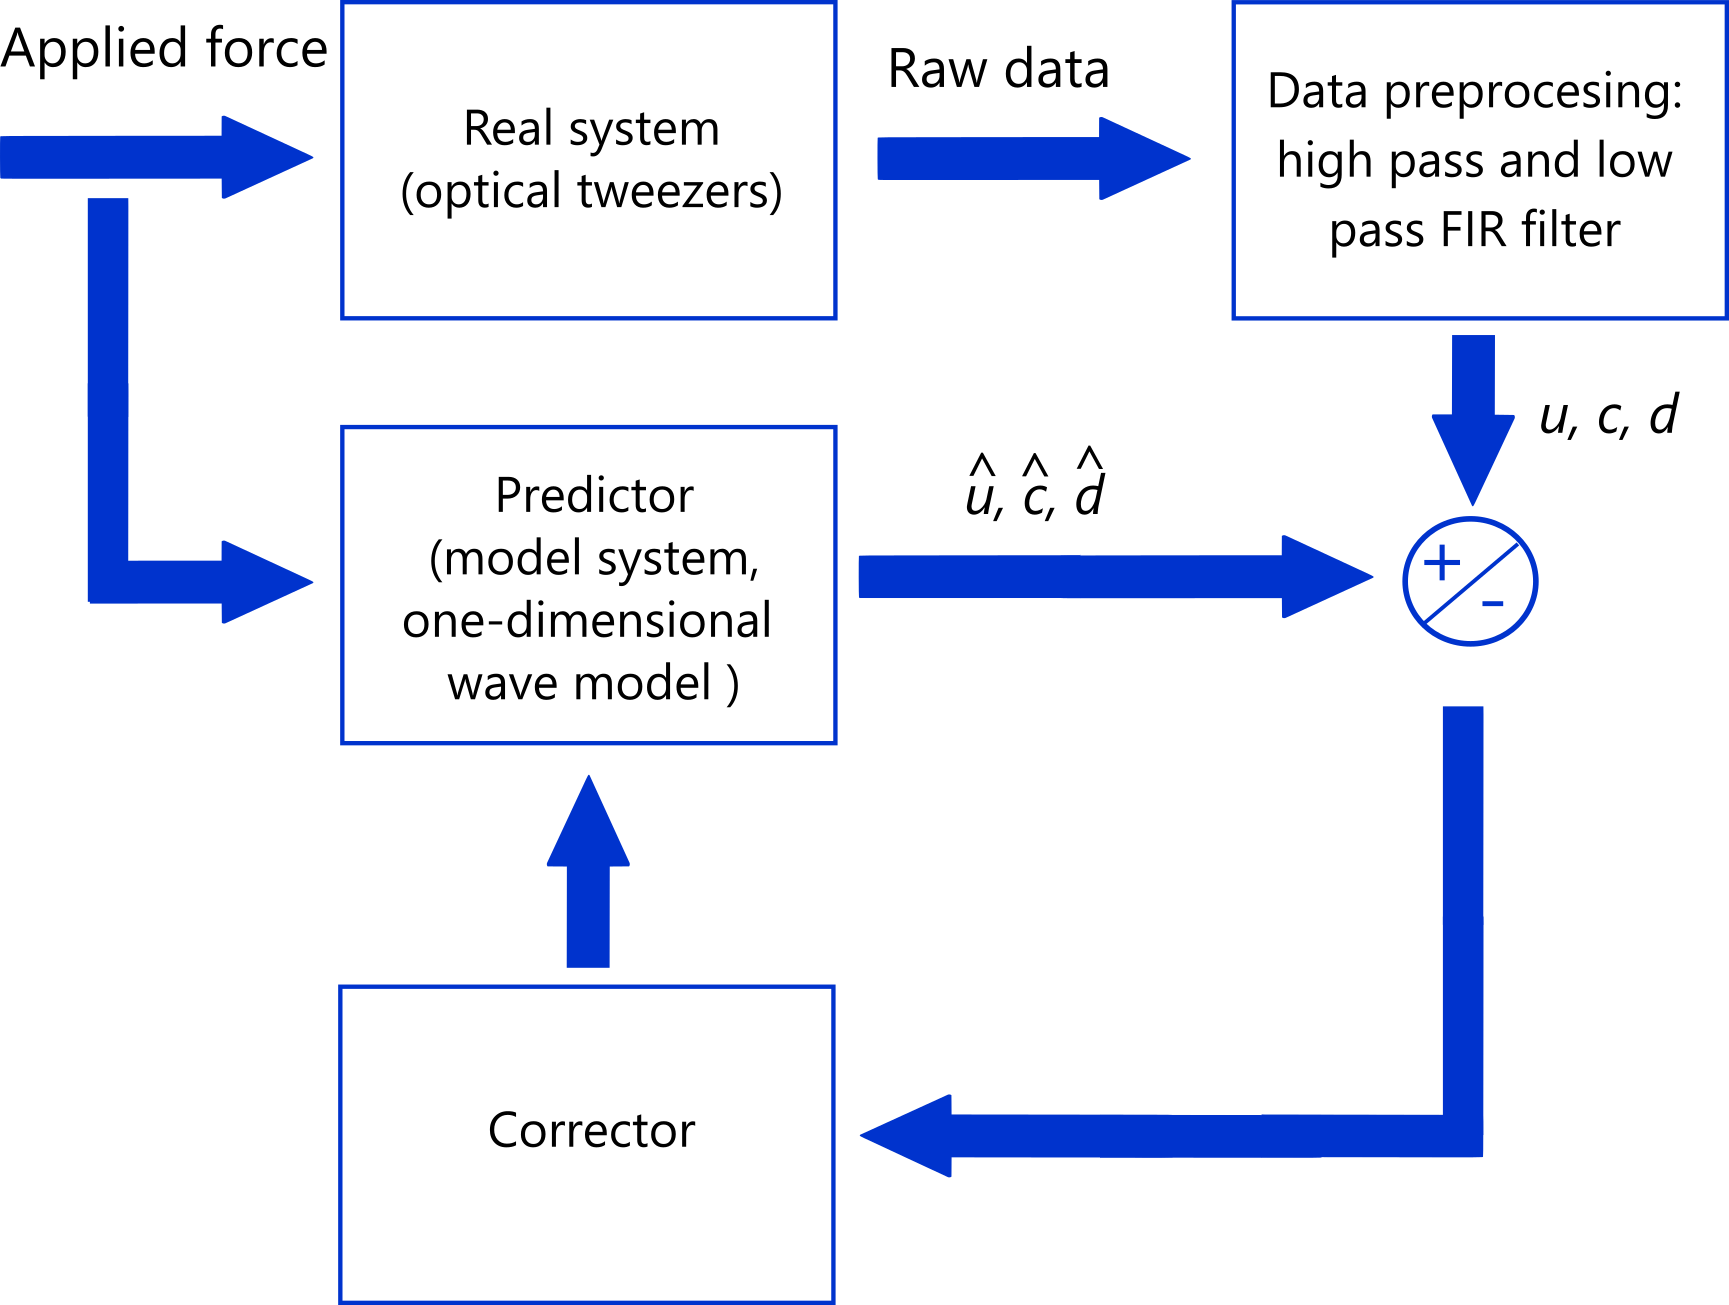
\includegraphics[width=0.65\textwidth]{figures/esquema_extended_kalman_filter.png}
	\caption{Block diagram of extended Kalman filter}
	\label{fig:kalman_esq}
\end{figure}

The equations that define the correction in the Extended Kalman filter are as follows:

\begin{equation} \label{eqn:corrector}
    \begin{array}{ l }
    
    Kk = P_{k}^{-}H^{T}[HP_{k}^{-}H^{T} + R]^{-1} \\
    \hat{Z_{k}} = \hat{Z_{k}^{-}} + Kk(y_{k}-H\hat{Z_{k}^{-})} \\
    P_{k} = (I - KkH)P_{k}^{-}
    
    \end{array}
\end{equation}

The correction of the extended Kalman filter is controlled by the Kalman gain, $Kk$, the parameter that regulates the difference between the a priori and the a posteriori estimated parameter. It is calculated with the covariance of the a priori estimated state,  $P_{k}^{-}$, a matrix with the sensor position, $H^{T}$, and the covariance of the sensor noise, $R$. The a posteriori estimated state, $\hat{Z_{k}}$, is obtained by multiplying the Kalman gain, $Kk$, by the difference between the matrix that indicates the sensor position, $H$, per the a priori estimated state, $\hat{Z_{k}^{-}}$, and the signal that has been captured by the sensor, $y_{k}$, and this value is added to the a priori estimated state,  $\hat{Z_{k}^{-}}$. A posteriori estimated state covariance, $P_{k}^{-}$, Kalman gain, $Kk$, sensor position matrix, $H$, and unitary matrix, $I$, are used to obtain the covariance of the estimated state, $P_{k}$.

These equations have been implemented in Matlab, where the function that defined the system was the wave equation in one dimension in polar coordinates as in the equation \ref{eqn:vk+1} and the force has been defined in the equation \ref{eqn:force}. 

The problem with this implementation of the extended Kalman filter is that it is a corrector, i.e., it is necessary to have an a priori value. The value of the initial position is 0 and then it is estimated with the model to which the filter has been coupled, however, it is necessary to determine an a priori value of the transmission velocity $c$ and the damping $d$. It is therefore necessary to analyse the performance of the extended Kalman filter in terms of how different the a priori values $c$ and $d$ are from the true value.

\setlength{\parskip}{0mm}

%%%%%%%%%%%%%%%%%%%%%%%%%%%%%%%%%%%%%%%%%%%%%%%%%%%%%%%%%%%%%%%%%%%%%%%%%%%%%%%%
\subsection{Validation}
%%%%%%%%%%%%%%%%%%%%%%%%%%%%%%%%%%%%%%%%%%%%%%%%%%%%%%%%%%%%%%%%%%%%%%%%%%%%%%%%

%%%%%%%%%%%%%%%%%%%%%%%%%%%%%%%%%%%%%%%%%%%%%%%%%%%%%%%%%%%%%%%%%%%%%%%%%%%%%%%%
\subsubsection{Obtain the real parameters}
%%%%%%%%%%%%%%%%%%%%%%%%%%%%%%%%%%%%%%%%%%%%%%%%%%%%%%%%%%%%%%%%%%%%%%%%%%%%%%%%

To validate the system it was necessary to merge the real data obtained with the computational system. To do this it was necessary to establish what the actual values were, which were then introduced into the computational model.

\setlength{\parskip}{4mm}

The initial step was to set a differential of time $dt$ and a differential of space $dx$ and $dr$ for the wave models. The differential of space, $dx$ and $dr$ has been calculated as follows:

\begin{equation} \label{eqn:dx}
	dx = dr = \frac{l}{n}
\end{equation}

The diameter of the cell nucleus was set as $l/2$. Since the two-dimensional wave model was solved on a square grid of nodes, in which the total number of nodes was $N$, the parameter $n$ was set as:

\begin{equation} \label{eqn:n}
	n = \sqrt{N}
\end{equation}

For one-dimensional simulations, the number of nodes $N$ was the parameter $n$. The differential time differential value $dt$ was determined using the position differential of position, $dx$ and the transmission velocity of the medium, $c$.

\begin{equation} \label{eqn:dt}
	dt = \frac{dx}{c}
\end{equation}

For this purpose, it was necessary to determine the transmission rate initial for the extended Kalman filter in the cell nucleus as shown below:

\begin{equation} \label{eqn:c}
	c = \sqrt{\frac{E}{p}}
\end{equation}

The parameter $E$ is Young's modulus, which can be obtained from the force contributed in an area, $\sigma$, and the proportional deformation of that area, $\epsilon$. The value of the initial Young's modulus has not been calculated in this work and depends on another project of the group. When that project is completed, the value obtained in this study will be used.

The parameter $p$ is the density, which has been estimated as the density of water \cite{patterson1994measurement}. 

The initial value of the damping has been proposed to be estimated in the following way, firstly the complex viscosity was obtained from the study of the microrheology \cite{el2008measuring}. 

\begin{equation} \label{eqn:microreology}
	\begin{array}{ l }
		
		G'(w) = \frac{F_{max}}{6\pi R x_{max}} cos(\Delta \theta) \\
		G''(w) = \frac{F_{max}}{6\pi R x_{max}} sin(\Delta \theta) \\
		\eta *(w) = [G'(w)^{2}+G'(w)^{2}]^{1/2}/w = [G'(w)^{2}+G'(w)^{2}]^{1/2}/2\pi f
		
	\end{array}
\end{equation}

For correlating damping with viscosity, the damped spring-mass model was used:

\begin{equation} \label{eqn:modelo_masa_resorte}
	\begin{array}{ l }
		
		m\ddot{x} - \xi \dot{x} = 0 \\
		\ddot{x} = \frac{\xi}{m^{3}p}\dot{x} \\
		b = \frac{\xi}{\bar{Vol} p} = \frac{\xi}{\Delta x p}
		
	\end{array}
\end{equation}

To obtain the value of $\xi$ , the Stokes problem was considered, in which there is a ball that has a frictional force..

\begin{equation} \label{eqn:stokes}
	F = 6\pi D \eta v = \xi v
\end{equation}

In this case, it was not a single sphere problem, but there were strands of chromatin in the nucleus, so the value of $\xi$ was obtained by calculating the fraction of the volume occupied by chromatin in the nucleus.

\begin{equation} \label{eqn:frac_nucl_chro}
	\Theta = \frac{Vol_{chromatin}}{Vol_{nucleus}} = \frac{\pi r_{c}^{2} l}{\frac{4\pi r_{n}^{3}}{3}}
\end{equation}

Thus, $\xi$ was approximated as:

\begin{equation} \label{eqn:xi_approx}
	\xi = \frac{\Delta x}{\Theta} \eta
\end{equation}

The force that generated the mechanical wave was obtained from the real data captured by the shaker trap and the real change of position was calculated with the data captured by the tactile trap. By using the elastic constant of the trap, $k$, a value obtained experimentally by the optical tweezers, the change of position, $u$, was obtained in the following way:

\begin{equation} \label{eqn:real_desp}
	u = \frac{\delta_{Fext}}{k}
\end{equation}

\newpage

%%%%%%%%%%%%%%%%%%%%%%%%%%%%%%%%%%%%%%%%%%%%%%%%%%%%%%%%%%%%%%%%%%%%%%%%%%%%%%%%
% RESULTS %
%%%%%%%%%%%%%%%%%%%%%%%%%%%%%%%%%%%%%%%%%%%%%%%%%%%%%%%%%%%%%%%%%%%%%%%%%%%%%%%%

\rhead{Results}
\section{Results}

\setlength{\parskip}{0mm}

%%%%%%%%%%%%%%%%%%%%%%%%%%%%%%%%%%%%%%%%%%%%%%%%%%%%%%%%%%%%%%%%%%%%%%%%%%%%%%%%
\subsection{Experimental desing}
%%%%%%%%%%%%%%%%%%%%%%%%%%%%%%%%%%%%%%%%%%%%%%%%%%%%%%%%%%%%%%%%%%%%%%%%%%%%%%%%

%%%%%%%%%%%%%%%%%%%%%%%%%%%%%%%%%%%%%%%%%%%%%%%%%%%%%%%%%%%%%%%%%%%%%%%%%%%%%%%%
\subsubsection{Jurkat cells, cell fragmentation and incubation with drug}
%%%%%%%%%%%%%%%%%%%%%%%%%%%%%%%%%%%%%%%%%%%%%%%%%%%%%%%%%%%%%%%%%%%%%%%%%%%%%%%%

The Jurkat cell has been fragmented to obtain the isolated nucleus. The images obtained of the isolated nuclei in the optical tweezers are shown below in figure \ref{fig:jurkat_cells} for an isolated nucleus, an isolated nucleus that was a control for the jasplakinolide experiment and a nucleus that has been incubated with the jasplakinolide drug.

\setlength{\parskip}{4mm}

\begin{figure}[htbp]
	\centering
	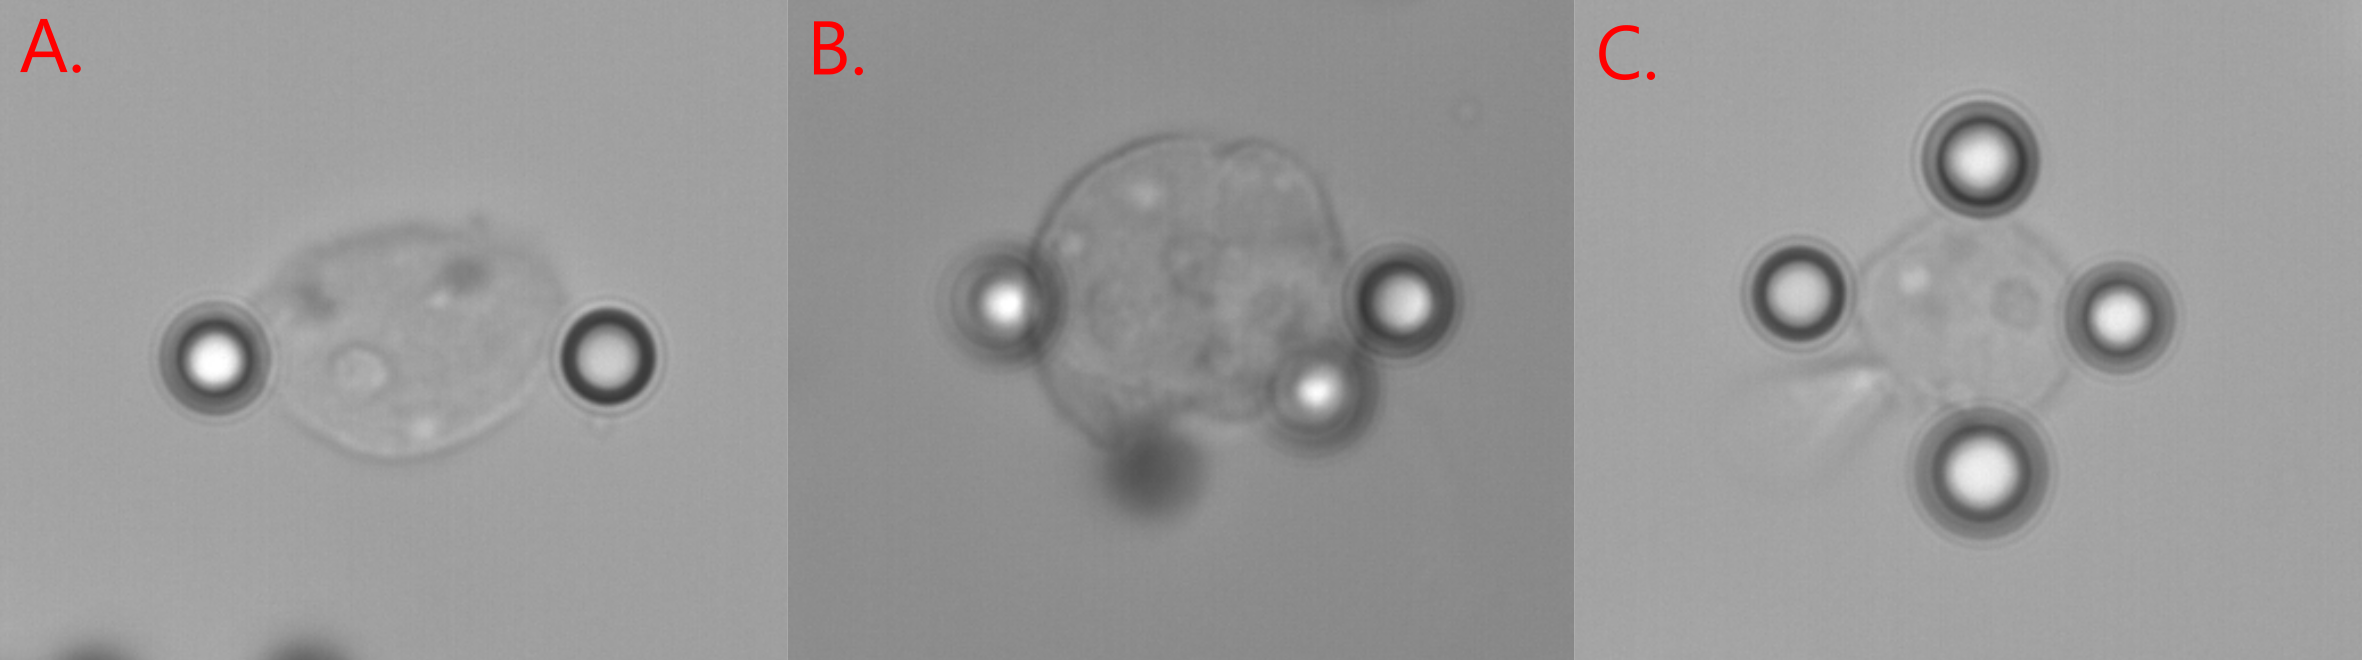
\includegraphics[width=0.9\textwidth]{figures/jurkat_cell_shape.png}
	\caption{A. Isolated Jurkat cell nucleus. B. Isolated Jurkat cell nucleus, jasplakinolide drug control. C. Isolated Jurkat cell nucleus incubated with jasplakinolide drug.}
	\label{fig:jurkat_cells}
\end{figure}

\setlength{\parskip}{0mm}

%%%%%%%%%%%%%%%%%%%%%%%%%%%%%%%%%%%%%%%%%%%%%%%%%%%%%%%%%%%%%%%%%%%%%%%%%%%%%%%%
\subsubsection{HeLa cells and incubation with beads}
%%%%%%%%%%%%%%%%%%%%%%%%%%%%%%%%%%%%%%%%%%%%%%%%%%%%%%%%%%%%%%%%%%%%%%%%%%%%%%%%

HeLa cells have been incubated with the beads in two possible approaches, the figure shows comparative images of a HeLa cell incubated in cell-culture treated multidishes and a cell incubated on the cover glass in an individual petri dish.

\setlength{\parskip}{4mm}

\begin{figure}[htbp]
	\centering
	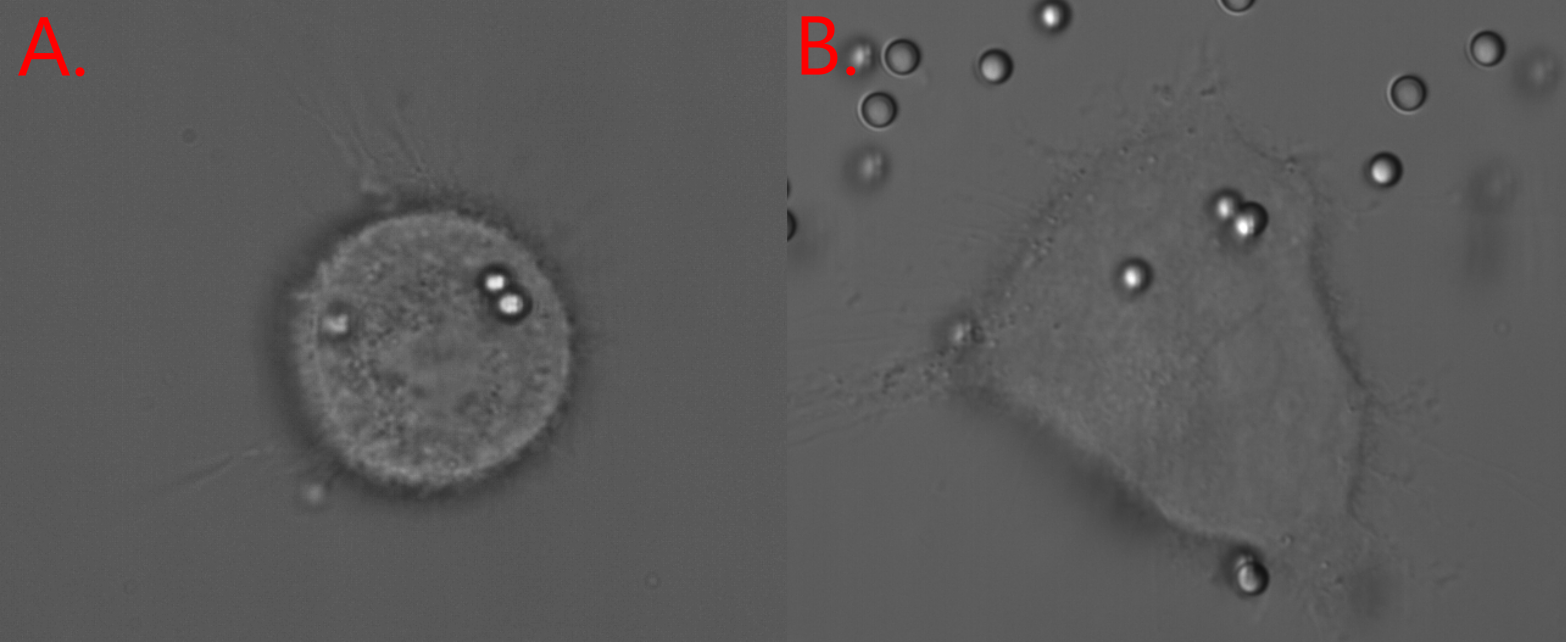
\includegraphics[width=0.60\textwidth]{figures/hela_cell_shape.png}
	\caption{A. HeLa cell incubated in cell-culture treated multidishes. B. HeLa cell incubated on the cover glass in an individual petri dish.}
	\label{fig:hela_cell_shape} 
\end{figure}

\setlength{\parskip}{0mm}

%%%%%%%%%%%%%%%%%%%%%%%%%%%%%%%%%%%%%%%%%%%%%%%%%%%%%%%%%%%%%%%%%%%%%%%%%%%%%%%%
\subsubsection{Identation of cell nucleus with optical tweezers}
%%%%%%%%%%%%%%%%%%%%%%%%%%%%%%%%%%%%%%%%%%%%%%%%%%%%%%%%%%%%%%%%%%%%%%%%%%%%%%%%

The nuclei of HeLa cells and Jurkat cells have been indented. A dataset of eight cells (two HeLa cells and six Jurkat cells), with a total of 54 indentations, was obtained. Some of the data captured with the optical tweezers traps are as follows:

\setlength{\parskip}{4mm}

\begin{figure}[htbp]
	\centering
	\includesvg[width=1\textwidth]{figures/datos_pinzas_no_filtrados_hela_jurkat.svg}
	\caption{Force values recorded on the optical tweezers. The first row corresponds to the identation in the nucleus of a HeLa cell and the second row to the identation in the isolated nucleus of a Jurkat cell.The first column corresponds to the beads that make identations and the second column to the beads that receive the signal at the other side of the nucleus. The frequency of the identations is 2Hz.}
	\label{fig:raw_data_cells}
\end{figure}

\setlength{\parskip}{0mm}

%%%%%%%%%%%%%%%%%%%%%%%%%%%%%%%%%%%%%%%%%%%%%%%%%%%%%%%%%%%%%%%%%%%%%%%%%%%%%%%%
\subsection{Computational desing}
%%%%%%%%%%%%%%%%%%%%%%%%%%%%%%%%%%%%%%%%%%%%%%%%%%%%%%%%%%%%%%%%%%%%%%%%%%%%%%%%

%%%%%%%%%%%%%%%%%%%%%%%%%%%%%%%%%%%%%%%%%%%%%%%%%%%%%%%%%%%%%%%%%%%%%%%%%%%%%%%%
\subsubsection{Preprocessing of the simulated data}
%%%%%%%%%%%%%%%%%%%%%%%%%%%%%%%%%%%%%%%%%%%%%%%%%%%%%%%%%%%%%%%%%%%%%%%%%%%%%%%%

A test has been carried out to check that the preprocessing algorithm works. To do this, a simulated signal (\ref{eqn:simulated_signal_preprocess}) in which the units are simulation units, has been created with the desired study frequency, 10Hz, and two frequencies associated with the noise of 2Hz and 24Hz. 

\setlength{\parskip}{4mm}

\begin{equation} \label{eqn:simulated_signal_preprocess}
	x = sin(2\pi\cdot 2t) + sin(2\pi\cdot 10t) + sin(2\pi\cdot 24t)
\end{equation}

A plot of the generated signal, the fourier transform, and the averaged fourier transform is shown below in figure \ref{fig:noisy_data_simulated}. Also, modelled signal was filtered using the high-pass and low-pass filter, obtaining the filtered signal shown below in figure \ref{fig:noisy_filtered_data_simulated}.

\begin{figure}[htbp]
	\centering
	\includesvg[width=0.9\textwidth]{figures/noisy_data_fourier_composition.svg}
	\caption{The first row shows the modelled signal with frequencies of 2, 10 and 24Hz. The second row shows firstly the Fourier transform frequency spectrum and secondly the averaged Fourier transform frequency spectrum.}
	\label{fig:noisy_data_simulated}
\end{figure}


\begin{figure}[htbp]
	\centering
	\includesvg[width=0.9\textwidth]{figures/noisy_data_fourier_composition_filter.svg}
	\caption{The first row shows the modelled signal with frequencies of 2, 10 and 24Hz filtered to remove frequencies below and above 10Hz. The second row shows firstly the Fourier transform frequency spectrum and secondly the averaged Fourier transform frequency spectrum.}
	\label{fig:noisy_filtered_data_simulated}
\end{figure}

\setlength{\parskip}{0mm}

\newpage
%%%%%%%%%%%%%%%%%%%%%%%%%%%%%%%%%%%%%%%%%%%%%%%%%%%%%%%%%%%%%%%%%%%%%%%%%%%%%%%%
\subsubsection{One-dimension wave model simulation}
%%%%%%%%%%%%%%%%%%%%%%%%%%%%%%%%%%%%%%%%%%%%%%%%%%%%%%%%%%%%%%%%%%%%%%%%%%%%%%%%

\setlength{\parskip}{0mm}

A one-dimensional wave has been obtained from the one-dimensional wave model in polar coordinates with Matlab. The units of the parameters are simulation units.

\setlength{\parskip}{4mm}

\begin{figure}[htbp]
    \centering
    \includesvg[width=0.5\textwidth]{figures/modelo_1d_sin_ruido_1.svg}
    \caption{Simulated wave captured by a sensor. It has been simulated with the 1-dimensional wave model in polar coordinates with Matlab.}
    \label{fig:modelo1}
\end{figure}

%%%%%%%%%%%%%%%%%%%%%%%%%%%%%%%%%%%%%%%%%%%%%%%%%%%%%%%%%%%%%%%%%%%%%%%%%%%%%%%%
\subsubsection{Two-dimension wave model simulation}
%%%%%%%%%%%%%%%%%%%%%%%%%%%%%%%%%%%%%%%%%%%%%%%%%%%%%%%%%%%%%%%%%%%%%%%%%%%%%%%%

\setlength{\parskip}{0mm}

From the two-dimensional wave model in polar coordinates implemented in Matlab, simulated data have been obtained. The values used in the simulation of this wave were the same as in figure \ref{fig:modelo1}. The graphs are presented in figure \ref{fig:modelo2}, the first graph is an ideal model without external noise, while in the second one there is a random noise of 40\%.

\setlength{\parskip}{4mm}

\begin{figure}[h!]
    \centering
    \includesvg[width=1\textwidth]{figures/modelo_2d_con_sin_ruido.svg}
    \caption{Simulated wave captured by a sensor. It has been simulated with the two-dimensional wave model in cartesian coordinates with Matlab. The first graph is an ideal model without noise and the second one has 40\% random noise.}
    \label{fig:modelo2}
\end{figure}

\newpage
%%%%%%%%%%%%%%%%%%%%%%%%%%%%%%%%%%%%%%%%%%%%%%%%%%%%%%%%%%%%%%%%%%%%%%%%%%%%%%%%
\subsubsection{Kalman filter analysis with simulated data}
%%%%%%%%%%%%%%%%%%%%%%%%%%%%%%%%%%%%%%%%%%%%%%%%%%%%%%%%%%%%%%%%%%%%%%%%%%%%%%%%

\setlength{\parskip}{0mm}

An analysis of the performance of the extended Kalman filter implemented in Matlab with equation systems \ref{eqn:predictor} and \ref{eqn:corrector} has been carried out. In all these simulations, the data obtained from the two-dimension model of figure \ref{fig:modelo2} have been used as real data and the data obtained from the one dimensional wave model in figure \ref{fig:modelo1} have been used as model data.

\setlength{\parskip}{4mm}

The figure \ref{fig:kalman1} shows the parameters obtained by the extended Kalman filter, the change in position, $u$, transmission velocity, $c$, and damping, $d$. In addition, the proposed initial values for propagation speed, $c$, and damping, $d$, are the real values.

\begin{figure}[h!]
    \centering
    \includesvg[width=1\textwidth]{figures/filtro_kalman_1_fixed.svg}
    \caption{Estimation of the change of position, transmission velocity and damping using the extended Kalman filter. The real data are simulated with two-dimensional wave model and the model data are obtained with one-dimensional wave model. The initial values for propagation speed and damping are the real values. In the first column the real data have no noise and in the second column they have 40\% random noise.}
    \label{fig:kalman1}
\end{figure}

To see the robustness of the extended Kalman filter depending on how close the proposed initial values of the transmission rate and damping are to the real ones, several tests have been performed changing the proposed initial value.  
First, figure \ref{fig:kalman1c} shows an initial value of the propagation velocity $c$ that is 25\% higher than the real one, that is an initial value of $1,25 c_{real}$.

\begin{figure}[h!]
    \centering
    \includesvg[width=1\textwidth]{figures/filtro_kalman_1_25_c_fixed.svg}
    \caption{Estimation of the change in position, transmission velocity and damping using the extended Kalman filter when the initial value of the propagation velocity is $1,25 c_{real}$. The real data are simulated using the two-dimensional wave model, the model data are obtained using the one-dimensional wave model. In the first column the real data has no noise and in the second column they have 40\% random noise.}
    \label{fig:kalman1c}
\end{figure}

Furthermore, the value of the parameters obtained with the extended Kalman filter is shown when the damping given at the beginning is $1,25 d_{real}$ in figure \ref{fig:kalman1d}.

\begin{figure}[h!]
    \centering
    \includesvg[width=1\textwidth]{figures/filtro_kalman_1_25_d_fixed.svg}
    \caption{Estimation of the change in position, transmission velocity and damping using the extended Kalman filter when the initial value of the damping, $d$, is $ 1,25 d_{real}$. The real data are simulated using the two-dimensional wave model, the model data are obtained using the one-dimensional wave model. In the first column the real data have no noise and in the second column they have 40\% random noise.}
    \label{fig:kalman1d}
\end{figure}

\newpage

As it is not usual to have the exact value of one parameter a priori and not of another, in figure \ref{fig:kalman1dc} an estimation of the parameters with Kalman filter is performed where the initial values of the propagation rate is $1,25 c_{real}$ and the damping is $1,25 d_{real}$.

\newpage

\begin{figure}[h!]
    \centering
    \includesvg[width=1\textwidth]{figures/filtro_kalman_1_25_c_d_fixed.svg}
    \caption{Estimation of the change in position, transmission velocity and damping using the extended Kalman filter when the initial value of the damping is $1,25 d_{real}$ and transmision velocity is $1,25 c_{real}$. The real data are simulated using the two-dimensional wave model, the model data are obtained using the one-dimensional wave model. In the first column the real data have no noise and in the second column they have 40\% random noise.}
    \label{fig:kalman1dc}
\end{figure}

Several simulations have been carried out with the extended Kalman filter to determine the final error of the parameters $c$ and $d$ as a function of the percentage difference between the initial value of the parameters and the actual value. The results of this analysis are presented the figure \ref{fig:valorescd}. The heat map shows if the final estimated value of the parameter is higher or lower than the real one, depending on the initial estimated parameter value is higher or lower than the real one. In addition, it is distinguished according to whether the system is noiseless or has 40\% random noise.

\begin{figure}[h!]
    \centering
    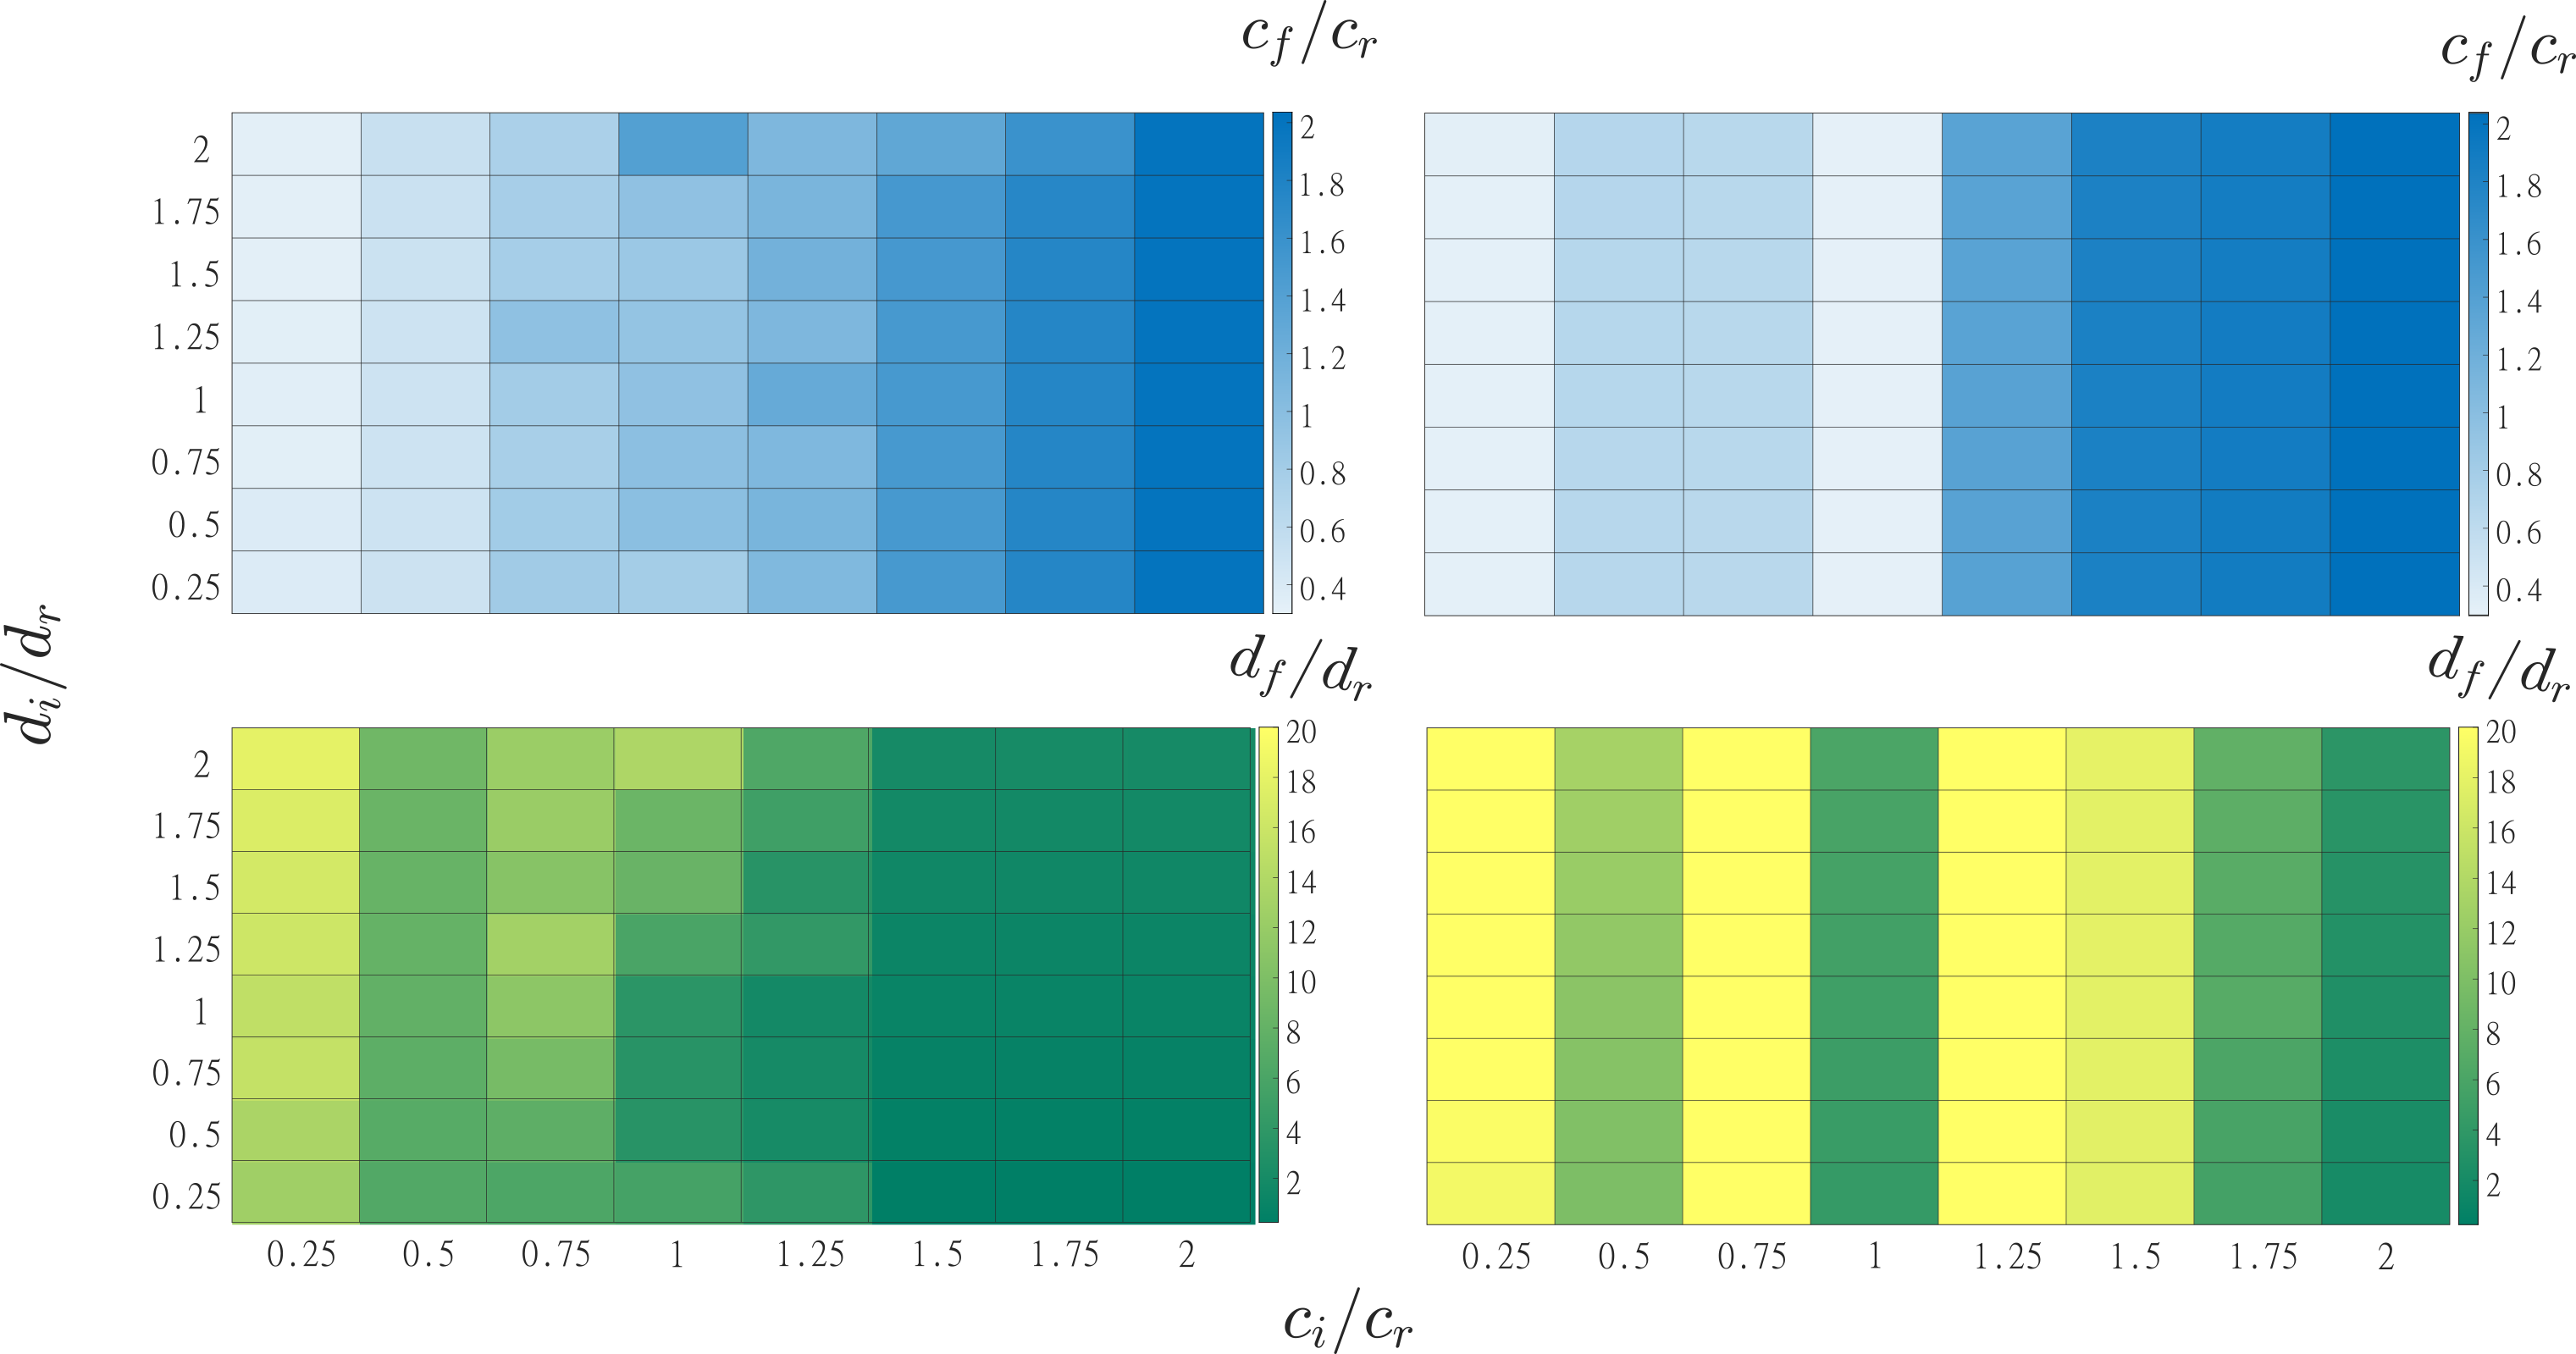
\includegraphics[width=1\textwidth]{figures/dependencia_valores_iniciales_1.png}
    \caption{Estimation of  transmission velocity and damping using the extended Kalman filter depending on the initial parameter value. The top row corresponds to the ratio between the final value and the real value of the transmission rate, while the second row corresponds to the ratio between the final value and the real value of the damping. The first column is obtained from values without noise, and the second column from real data (obtained from the two-dimensional wave model) with 40\% random noise.}
    \label{fig:valorescd}
\end{figure}

\newpage

\setlength{\parskip}{0mm}

%%%%%%%%%%%%%%%%%%%%%%%%%%%%%%%%%%%%%%%%%%%%%%%%%%%%%%%%%%%%%%%%%%%%%%%%%%%%%%%%
\subsection{Validation}
%%%%%%%%%%%%%%%%%%%%%%%%%%%%%%%%%%%%%%%%%%%%%%%%%%%%%%%%%%%%%%%%%%%%%%%%%%%%%%%%

%%%%%%%%%%%%%%%%%%%%%%%%%%%%%%%%%%%%%%%%%%%%%%%%%%%%%%%%%%%%%%%%%%%%%%%%%%%%%%%%
\subsection{Pre-processing of real data}
%%%%%%%%%%%%%%%%%%%%%%%%%%%%%%%%%%%%%%%%%%%%%%%%%%%%%%%%%%%%%%%%%%%%%%%%%%%%%%%%

\begin{wrapfigure}{r}{0.5\linewidth}
    \centering
    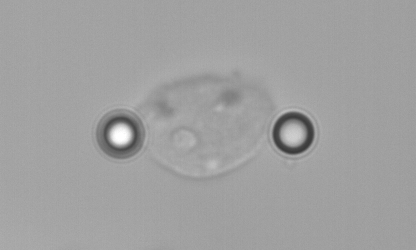
\includegraphics[width=0.45\textwidth]{figures/recorte_nucleo.png}
    \caption{Isolated nucleus of a Jurkat cell in which one bead was being indented while another bead received the signal}
    \label{fig:myfig3}
\end{wrapfigure}

Real data have been obtained by embedding a bead in a cell nucleus while another bead captured the waves at the other edge of the nucleus. The results presented have been obtained from the image \ref{fig:myfig3}, a isolated Jurkat cell nucleus. It has been indented with a force amplitude of 0,5$\mu$m and frequencies of 2Hz, 4Hz, 5Hz, 8Hz, and 10Hz for 30 seconds. Figure \ref{fig:raw_data} have several graphs which compare the force emitted by the identing bead and the force that reaches the bead sensor. \\

\setlength{\parskip}{4mm}

\begin{figure}[htbp]
  \centering
  \includesvg[width=1\textwidth]{figures/raw_data_graph_2.svg}
  \caption{Force captured by the optical tweezers during identation of a isolated Jurkat cell nucleus. The first column corresponds to the beads that make identations and the second column to the beads that receive the signal at the other side of the nucleus. The frequency of the identations was 2Hz in the first row, 5Hz in the second row and 10Hz in the third row.}
  \label{fig:raw_data}
\end{figure}

As the values captured by the force sensor of the optical tweezers were noisy, a filtering was performed. An averaged fast Fourier transform was used to determine the frequencies corresponding to the noise. Although the force values collected by the bead performing the identations had noise, only the fast Fourier transform and averaged fast Fourier transform of the beads acting as sensors are shown in figure \ref{fig:fourier_sin_filtro}, as these values were the most affected by noise. 

\newpage

\begin{figure}[htbp]
  \centering
  \includesvg[width=0.70\textwidth]{figures/transformada_fourier_limpia.svg}
  \caption{Fast Fourier transforms and the average of the fast Fourier transform of the signal captured by the tactile trap. The first column corresponds to the fast Fourier transform and the second to the average of the fast Fourier transform in which the mean has been averaged over two-cycle data sets. The frequencies applied in the indentation were 2Hz in the first row, 5Hz in the second row and 10Hz in the third row.}
  \label{fig:fourier_sin_filtro}
\end{figure}

Then, these signals were filtered using the low pass and high pass finite impulse response filter to obtain the filtered forces shown in figure \ref{fig:filtered_data}. Moreover, the Fourier transform and the average of the Fourier transform were also performed to verify that the signal has been filtered by removing high and low frequency noise with the low pass and high pass FIR filter. Both Fourier transforms are plotted in the figure \ref{fig:fourier_con_filtro_todo}.

With this analysis, the preprocessing of the real data was finished and the force captured by the optical tweezers was stored filtered.

\newpage

\begin{figure}[htbp]
  \centering
  \includesvg[width=1\textwidth]{figures/filtered_data_graph_2.svg}
  \caption{Force captured by the optical tweezers during identation, filtered with the high pass and low pass FIR filter. The first column corresponds to the beads that make identations and the second column to the beads that receive the signal at the other side of the nucleus. The frequency of the identations was 2Hz in the first row, 5Hz in the second row and 10Hz in the third row.}
  \label{fig:filtered_data}
\end{figure}

\begin{figure}[H]
    \centering
    \includesvg[width=0.7\textwidth]{figures/fourier_datos_pinzas_filtrados_fixed.svg}
  \caption{Force captured by the optical tweezers during identation filtered with the high pass and low pass FIR filter. The first column corresponds to the beads that make identations and the second column to the beads that receive the signal at the other side of the nucleus. The frequency of the identations was 2Hz in the first row, 5Hz in the second row and 10Hz in the third row.}
  \label{fig:fourier_con_filtro_todo}
\end{figure}

\newpage

%%%%%%%%%%%%%%%%%%%%%%%%%%%%%%%%%%%%%%%%%%%%%%%%%%%%%%%%%%%%%%%%%%%%%%%%%%%%%%%%
% DISCUSSION %
%%%%%%%%%%%%%%%%%%%%%%%%%%%%%%%%%%%%%%%%%%%%%%%%%%%%%%%%%%%%%%%%%%%%%%%%%%%%%%%%

\rhead{Discussion}
\section{Discussion}

%%%%%%%%%%%%%%%%%%%%%%%%%%%%%%%%%%%%%%%%%%%%%%%%%%%%%%%%%%%%%%%%%%%%%%%%%%%%%%%%
\subsection{Experimental desing}
%%%%%%%%%%%%%%%%%%%%%%%%%%%%%%%%%%%%%%%%%%%%%%%%%%%%%%%%%%%%%%%%%%%%%%%%%%%%%%%%

%%%%%%%%%%%%%%%%%%%%%%%%%%%%%%%%%%%%%%%%%%%%%%%%%%%%%%%%%%%%%%%%%%%%%%%%%%%%%%%%
\subsubsection{Jurkat cells, cell fragmentation and incubation with drug}
%%%%%%%%%%%%%%%%%%%%%%%%%%%%%%%%%%%%%%%%%%%%%%%%%%%%%%%%%%%%%%%%%%%%%%%%%%%%%%%%

\setlength{\parskip}{0mm}

First, the Jurkat cell nuclei were isolated correctly as the methodology was optimized. However, it was important to perform the indentation on the same day as the extraction because if they were stored in the eppendorf in which the extraction was performed, they would stick together and it was difficult to resuspend them.

\setlength{\parskip}{4mm} 

Also, it was expected that over time the cell nuclei would start to degrade and therefore the mechanical properties of the cell nuclei would change. It could be an interesting experiment to determine the lifetime of the isolated nuclei to perform indentation with them, in which they not only remain unbroken, but the mechanical properties they exhibit change as little as possible and are recognisable.

On the other hand, the concentration of drug that was used degraded most nuclei and it was quite difficult to find unbroken nuclei. Perhaps it would be better to use a lower drug concentration or the same drug concentration for a shorter time. 

%%%%%%%%%%%%%%%%%%%%%%%%%%%%%%%%%%%%%%%%%%%%%%%%%%%%%%%%%%%%%%%%%%%%%%%%%%%%%%%%
\subsubsection{HeLa cells and incubation with beads}
%%%%%%%%%%%%%%%%%%%%%%%%%%%%%%%%%%%%%%%%%%%%%%%%%%%%%%%%%%%%%%%%%%%%%%%%%%%%%%%%

\setlength{\parskip}{0mm}

As the long-term goal is to obtain measurements of the mechanical properties of the nucleus in living cells, it is important to optimise the phagocytosis of the beads in the cells. In this case, experiments have been performed with Hela cells, with which several factors have been determined that could influence bead internalisation. On the one hand, it is necessary to have a high concentration of cells when the incubation is started, because when the beads were added, the cells grew worse and divided less. It is also important that the medium is changed when the beads are added, firstly to have a better control of the percentage of beads in the medium and secondly, if the medium has been used for more than two days, it has been observed that the beads are barely internalised. It also seems that if they have been attached to the substrate for a short time (24 hours), more beads are internalised and this could happen because they are adherent cells that tend to extend, which could cause that the cell membrane is too tense to internalise the beads. It is important to carry out a more detailed study in the future in which cells that have internalised beads and those that have not are counted to optimise this methodology.

\setlength{\parskip}{4mm}

In addition, incubation of the cells on the cover glass in an individual petri dish has the advantage that the cells are attached and not in suspension, so there is no need to wait for them to re-attach to the cover glass as those in the multidishes that need to be detached, because the indentation cannot be performed correctly if the cell is sinking. In addition, the properties of the nucleus may change if it is unattached, attaching and already attached, which requires additional control.

%%%%%%%%%%%%%%%%%%%%%%%%%%%%%%%%%%%%%%%%%%%%%%%%%%%%%%%%%%%%%%%%%%%%%%%%%%%%%%%%
\subsubsection{Identation of cell nucleus with optical tweezers}
%%%%%%%%%%%%%%%%%%%%%%%%%%%%%%%%%%%%%%%%%%%%%%%%%%%%%%%%%%%%%%%%%%%%%%%%%%%%%%%%

\setlength{\parskip}{0mm}

Indentation in the optical tweezers has been performed on isolated Jurkat cell nuclei and HeLa nuclei with different results.

\setlength{\parskip}{4mm}

On the one hand, indentations on single nuclei of Jurkat cells have been successfully performed by obtaining data on the force produced on one side of the nucleus and the force transmitted to the other side of the nucleus. However, this was only possible with 3$\mu$m beads, as 2$\mu$m beads were very difficult to trap. 

On the other hand, no results have been obtained with HeLa cells. Indentations were made with the shaker trap, but the tactile bead did not register the force after passing through the nucleus. This may happen because 2$\mu$m beads were used, which were later discovered that they are poorly trapped, and they were apparently trapped in the cell but in fact were not, or it maybe they were not close enough to the nucleus for either of the two beads. 

An important difference between the two experiments is that in the Jurkat cells, the shaker trap was able to perform a higher force while in the HeLa cells the beads were in a vesicle inside the cell, where it could hardly move and produced a lower force. In addition, this probably contributed to the non-capture of the force in the tactile trap of the HeLa cell.

Perhaps in order to perform force detection correctly in the Hela cell it is necessary to internalise 3$\mu$m beads which are better captured,

%%%%%%%%%%%%%%%%%%%%%%%%%%%%%%%%%%%%%%%%%%%%%%%%%%%%%%%%%%%%%%%%%%%%%%%%%%%%%%%%
\subsection{Computational desing}
%%%%%%%%%%%%%%%%%%%%%%%%%%%%%%%%%%%%%%%%%%%%%%%%%%%%%%%%%%%%%%%%%%%%%%%%%%%%%%%%

%%%%%%%%%%%%%%%%%%%%%%%%%%%%%%%%%%%%%%%%%%%%%%%%%%%%%%%%%%%%%%%%%%%%%%%%%%%%%%%%
\subsubsection{Preprocessing of the simulated data}
%%%%%%%%%%%%%%%%%%%%%%%%%%%%%%%%%%%%%%%%%%%%%%%%%%%%%%%%%%%%%%%%%%%%%%%%%%%%%%%%

\setlength{\parskip}{0mm}

To check that the data pre-processing algorithm works correctly, it was tested with a simulated signal. The simulated signal was composed of three sine components with different frequencies, which results in an apparently very noisy signal. The fast Fourier transform and the averaged fast Fourier transform showed the three frequencies of the signal, however, the averaged one has a smaller number of values in the representation. This signal was processed with the high pass and low pass FIR filter, removing frequencies above and below 10Hz. The signal showed flattened maxima and peaked minima, a perfect signal was not obtained, however, with the fast Fourier transform and the averaged fast Fourier transform it can be seen that the only frequency of the signal was the desired one. In both transforms it was observed that the 10Hz peak lost a little intensity and in the averaged one the close frequencies were observed with a little intensity. This could be due to artefacts in the averaging or because the reduction of higher and lower frequencies did not result in a perfect signal and this is due to the maxima and minima, which did not have the shape of a perfect curve, but instead had straight lines and peaks.

\setlength{\parskip}{4mm}

%%%%%%%%%%%%%%%%%%%%%%%%%%%%%%%%%%%%%%%%%%%%%%%%%%%%%%%%%%%%%%%%%%%%%%%%%%%%%%%%
\subsubsection{One-dimension wave model simulation}
%%%%%%%%%%%%%%%%%%%%%%%%%%%%%%%%%%%%%%%%%%%%%%%%%%%%%%%%%%%%%%%%%%%%%%%%%%%%%%%%


\setlength{\parskip}{0mm}

\setlength{\parskip}{4mm}

%%%%%%%%%%%%%%%%%%%%%%%%%%%%%%%%%%%%%%%%%%%%%%%%%%%%%%%%%%%%%%%%%%%%%%%%%%%%%%%%
\subsubsection{Two-dimension wave model simulation}
%%%%%%%%%%%%%%%%%%%%%%%%%%%%%%%%%%%%%%%%%%%%%%%%%%%%%%%%%%%%%%%%%%%%%%%%%%%%%%%%


\setlength{\parskip}{0mm}

\setlength{\parskip}{4mm}

%%%%%%%%%%%%%%%%%%%%%%%%%%%%%%%%%%%%%%%%%%%%%%%%%%%%%%%%%%%%%%%%%%%%%%%%%%%%%%%%
\subsubsection{Kalman filter analysis with simulated data}
%%%%%%%%%%%%%%%%%%%%%%%%%%%%%%%%%%%%%%%%%%%%%%%%%%%%%%%%%%%%%%%%%%%%%%%%%%%%%%%%


\setlength{\parskip}{0mm}

\setlength{\parskip}{4mm}

%%%%%%%%%%%%%%%%%%%%%%%%%%%%%%%%%%%%%%%%%%%%%%%%%%%%%%%%%%%%%%%%%%%%%%%%%%%%%%%%
\subsection{Validation}
%%%%%%%%%%%%%%%%%%%%%%%%%%%%%%%%%%%%%%%%%%%%%%%%%%%%%%%%%%%%%%%%%%%%%%%%%%%%%%%%

%%%%%%%%%%%%%%%%%%%%%%%%%%%%%%%%%%%%%%%%%%%%%%%%%%%%%%%%%%%%%%%%%%%%%%%%%%%%%%%%
\subsubsection{Pre-processing of real data}
%%%%%%%%%%%%%%%%%%%%%%%%%%%%%%%%%%%%%%%%%%%%%%%%%%%%%%%%%%%%%%%%%%%%%%%%%%%%%%%%

\setlength{\parskip}{0mm}

\setlength{\parskip}{4mm}

\newpage

%%%%%%%%%%%%%%%%%%%%%%%%%%%%%%%%%%%%%%%%%%%%%%%%%%%%%%%%%%%%%%%%%%%%%%%%%%%%%%%%
% BIBLIOGRAPHY %
%%%%%%%%%%%%%%%%%%%%%%%%%%%%%%%%%%%%%%%%%%%%%%%%%%%%%%%%%%%%%%%%%%%%%%%%%%%%%%%%
\spacing{1}
\pagestyle{empty}
\bibliographystyle{ieeetr}
\bibliography{Bibliography.bib}

\newpage
%%%%%%%%%%%%%%%%%%%%%%%%%%%%%%%%%%%%%%%%%%%%%%%%%%%%%%%%%%%%%%%%%%%%%%%%%%%%%%%%
% APPENDIX %
%%%%%%%%%%%%%%%%%%%%%%%%%%%%%%%%%%%%%%%%%%%%%%%%%%%%%%%%%%%%%%%%%%%%%%%%%%%%%%%%
\setlength{\parskip}{0mm}
\section{Appendix}

\subsection{Buffer A recipe}

The recipe for 10 ml of buffer A is as follows: 8,79 ml of distilled water, 100$\mu$l of 1M solution of HEPES pH 8,0 (Sigma-Aldrich/FR), 33,2$\mu$l of 3M KCl solution (Carlo Erba/FR), 15$\mu$l of MgCl$_{2}$ solution (Calbiochem/DE), 1,162g of sucrose (Riedel-de Haën/DE), 1ml of 10\% glycerol (Sigma-Aldrich/MY), 50$\mu$l of 200mM DTT solution (BioRad/CA) and 10$\mu$l of 100\% Triton x-100 (Sigma-Aldrich/USA). To obtain a HEPES solution at pH 8.0, it was necessary to use a Hach Basic 20+ ph meter, where a 5M NaOH solution (Fine Chemicals/ZA) was added to the 1M HEPES solution until pH 8.0 was obtained. These solutions were collected in a Falcon conical tube of 15ml capacity. 

\subsection{TKM recipe}

The recipe to make 10ml of TKM buffer is as follows: 9,86ml of distilled water, 33,2$\mu$l of 3M KCl solution (Carlo Erba/FR), 19$\mu$l of 1M MgCl$_{2}$ solution (Calbiochem/DE) and 100$\mu$l of tris(hydroxymehtyl)aminomethane hydrochloride buffer substance pH 7,4 (Fluka Analytical/USA). These solutions were mixed in a Falcon conical tube of 15ml capacity.

\subsection{Jasplakinolide recipe}

The recipe to make 1ml of 100$\mu$g/ml jasplakinolide solution is as follows: 1ml of DMSO (Merk/DE) and 100$\mu$g of Jasplakinolide (Sigma-Aldrich/USA).




\end{document}

